
\subsection{ABC-Flow model fitting }

In order to characterise the~\textcite{Litcofsky:2012gr} toggle switch, I use the data collected in Section~\ref{sec:ts_time} to fit the~\textcite{Gardner:2000vha} toggle switch model, shown in Section (XXX). In order to do that, I use ABC-Flow as described in the Methods in Section~\ref{sec:abcflow-meth}.

%Prior to using ABC-Flow to fit the experimental data to a toggle switch model, ABC-Flow must be validated. In the following sections I first use randomly generated distributions to set the algorithm metrics and distances. Then I use a simulated data set to which I fit a toggle switch model and finally I use ABC-Flow to fit experimental data.  

In the following sections I first use normal distributions to study the distance functions used in ABC-Flow. Then I use a simulated data set to which I fit a toggle switch model and finally I use ABC-Flow to fit experimental data.  

\subsubsection{Distance study}
%Here I simulate two normal distributions, with identical mu and sigma, and calculate the distance between the two using the distance measure used in ABC-Flow. Doing this 1000 times, we then plot the distribution of epsilon. By doing that we can calculate the variance of the epsilon distribution, and find out the error that can be expected when measuring the distance in ABC-Flow. By doing that in 1D and in 2D we can compare the epsilon variances. 

Here, I simulate two normal distributions, with $\mu=0$ and $\sigma=1$ and measure the distance between them using the Kolmogorov-Smirnov test, as used in ABC-Flow. Doing this multiple times, the expected variation in distance values for identical distributions can be calculated. This is the error that can be expected when measuring distance in ABC-Flow. As can be seen in Figure~\ref{fig:epsilon_boxplt}, there range of distance values obtained in the 1D case is small, as the distance between two data sets drawn from the same distribution ranges from 0.1 to 0.2. For the 2D case, the distance values obtained vary more than in the 1D case. 


\begin{figure}[htbp]
\centering
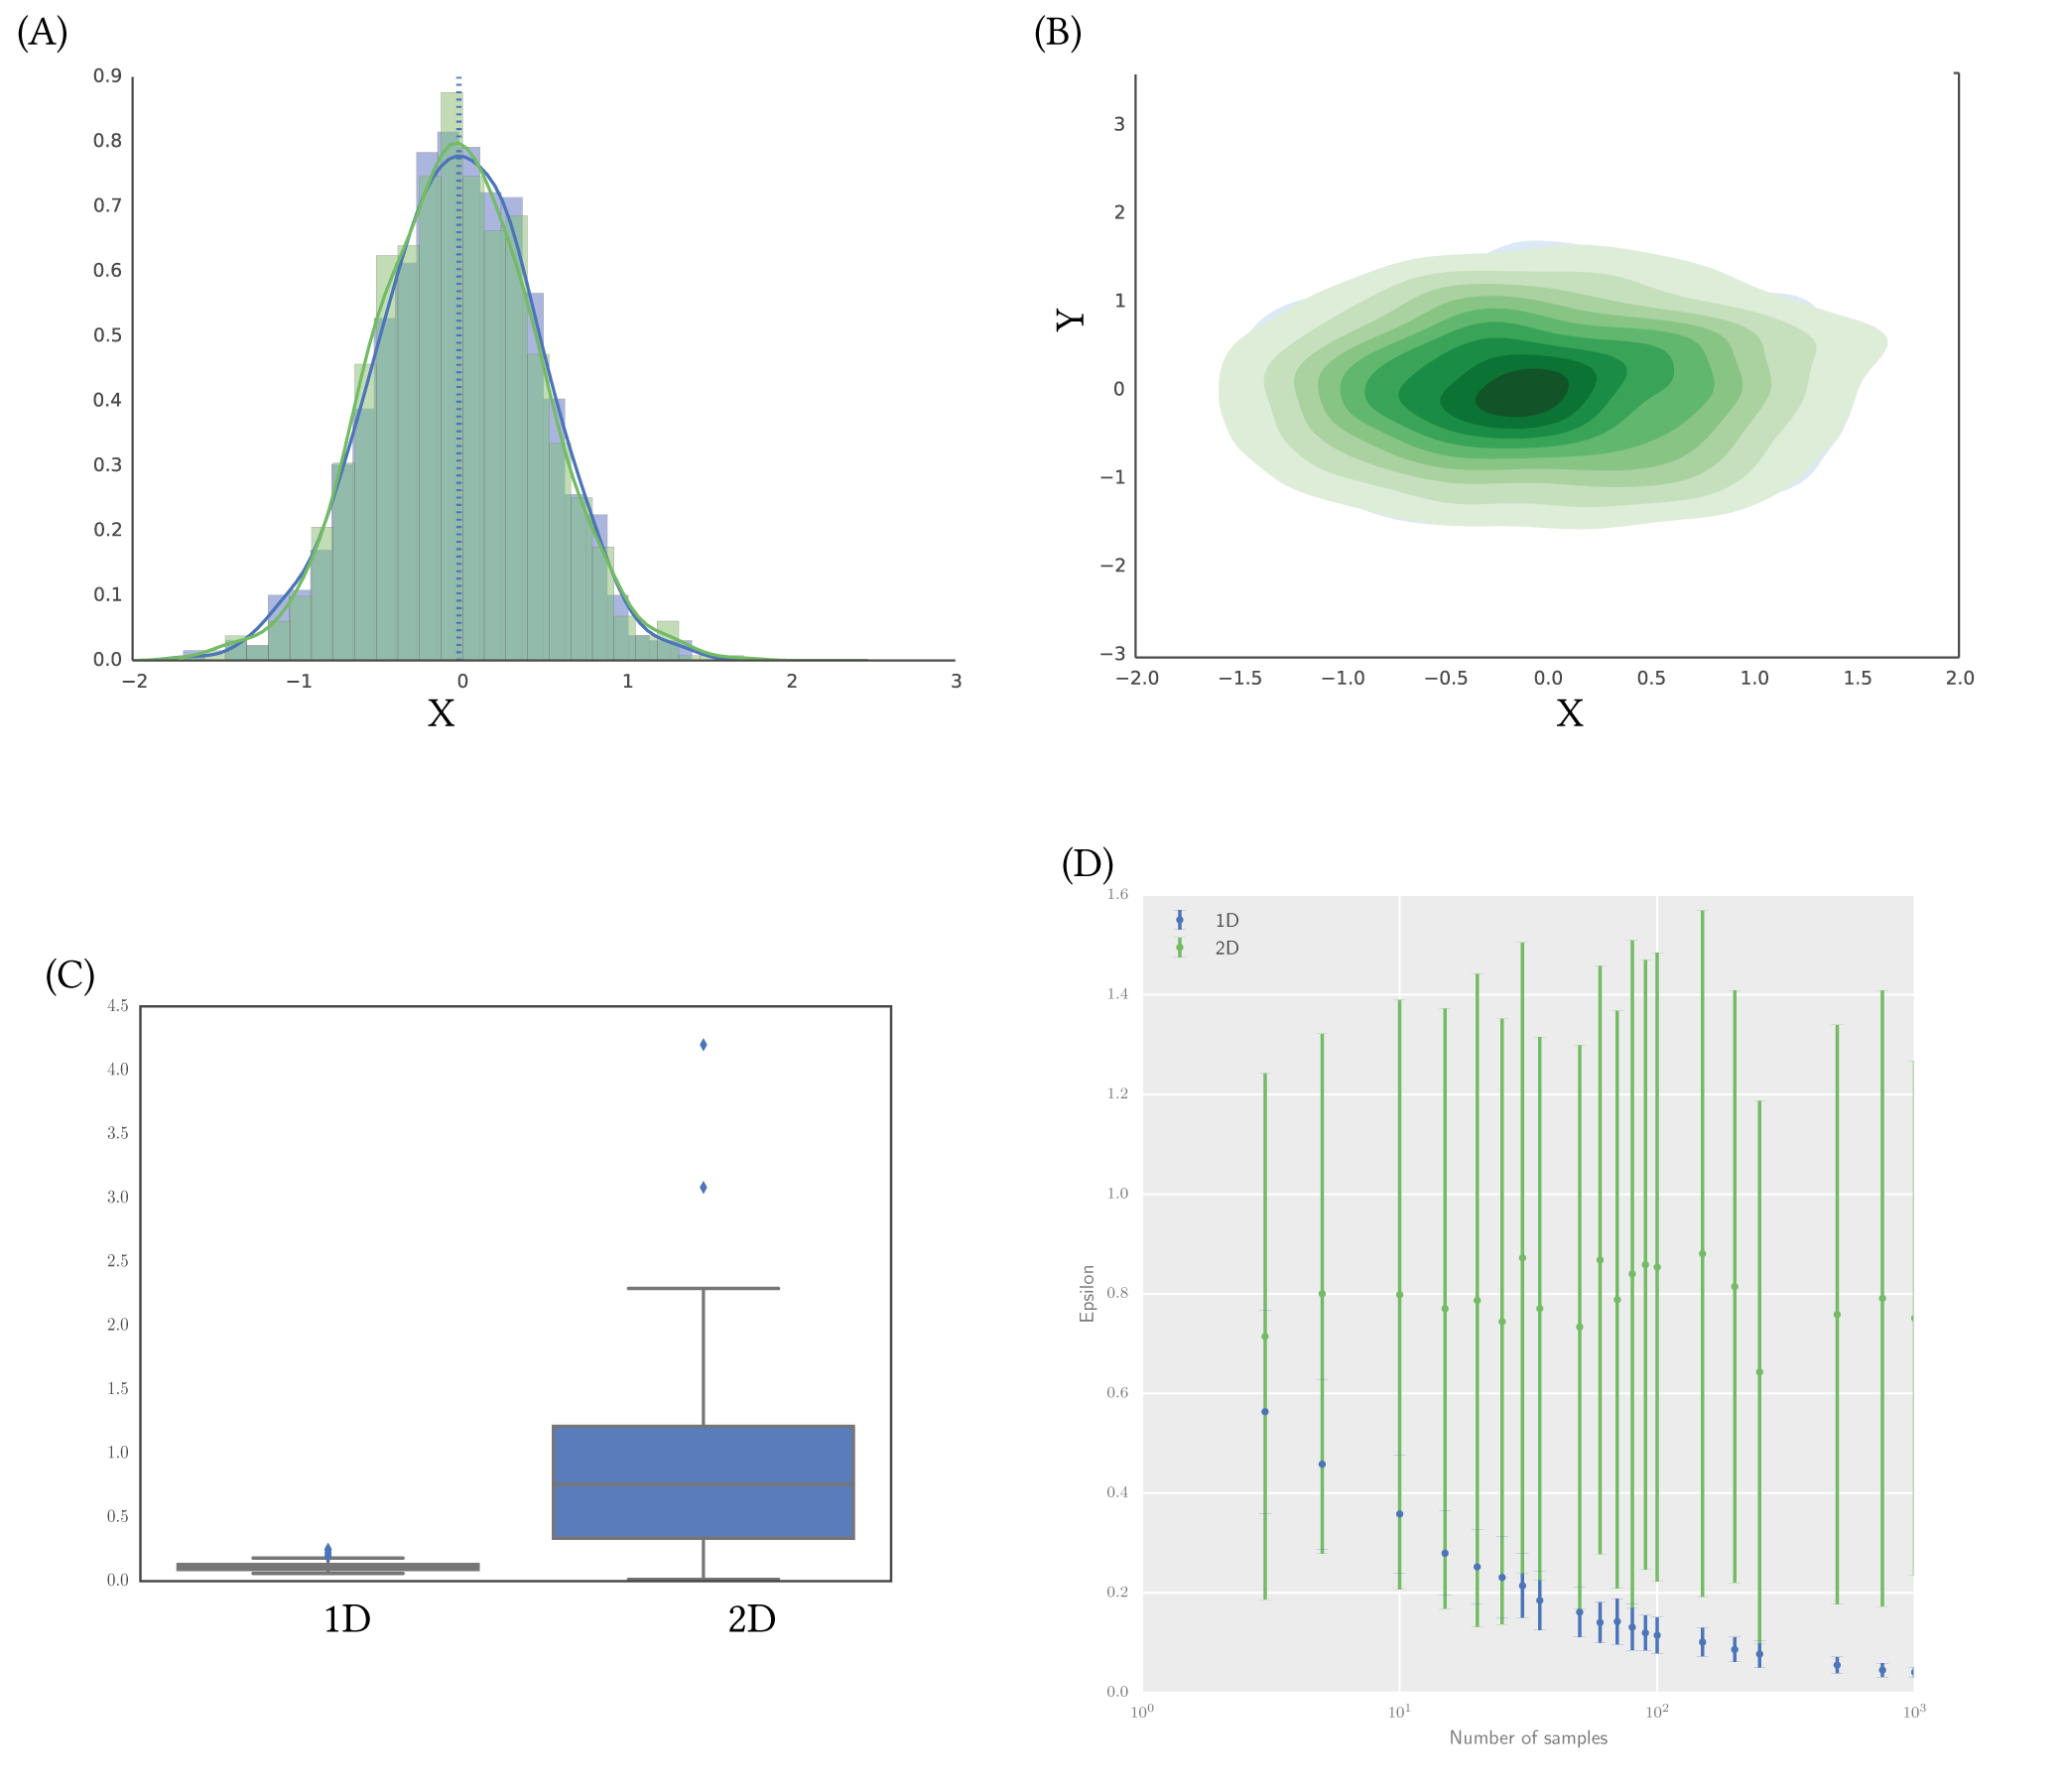
\includegraphics[scale=0.7]{chapterABCFlow/images/epsilon_same_box.png}
\caption[LoF caption]{\label{fig:epsilon_boxplt} The distance between two data sets drawn form the same distribution are compared using the Kolmogorov-Smirnov two sample test. (A) in 1D and (B) in 2D. (C) The distance is calculated for 1000 data sets. A greater variation of values is found for the 2D distance calculation.  }
\label{fig:normal_example}
\end{figure}
\clearpage


To further study the distance calculation used in ABC-Flow, the data sets are drawn from increasingly different distributions, and the distance between them calculated. As shown in Figure~\ref{fig:epsilon_mud}, the 1D distance is 0 when the difference between the \textmu{} from which the two datasets are drawn is 0.5 or less, and 1 when the difference in the \textmu{} between the two data sets is 7 or larger. In the 2D case the standard deviation of the calculated distance is larger than the 1D case. The distance calculation reaches a plateau at epsilon = 2.3 when the \textmu{} difference is 3 or larger. As shown in Figure~\ref{fig:epsilon_mud}D, as the number of samples drawn from each distribution increases, the standard deviation of the distance calculations decreases in the 1D case. This trend is less obvious in the 2D case.
\begin{figure}[htbp]
\centering
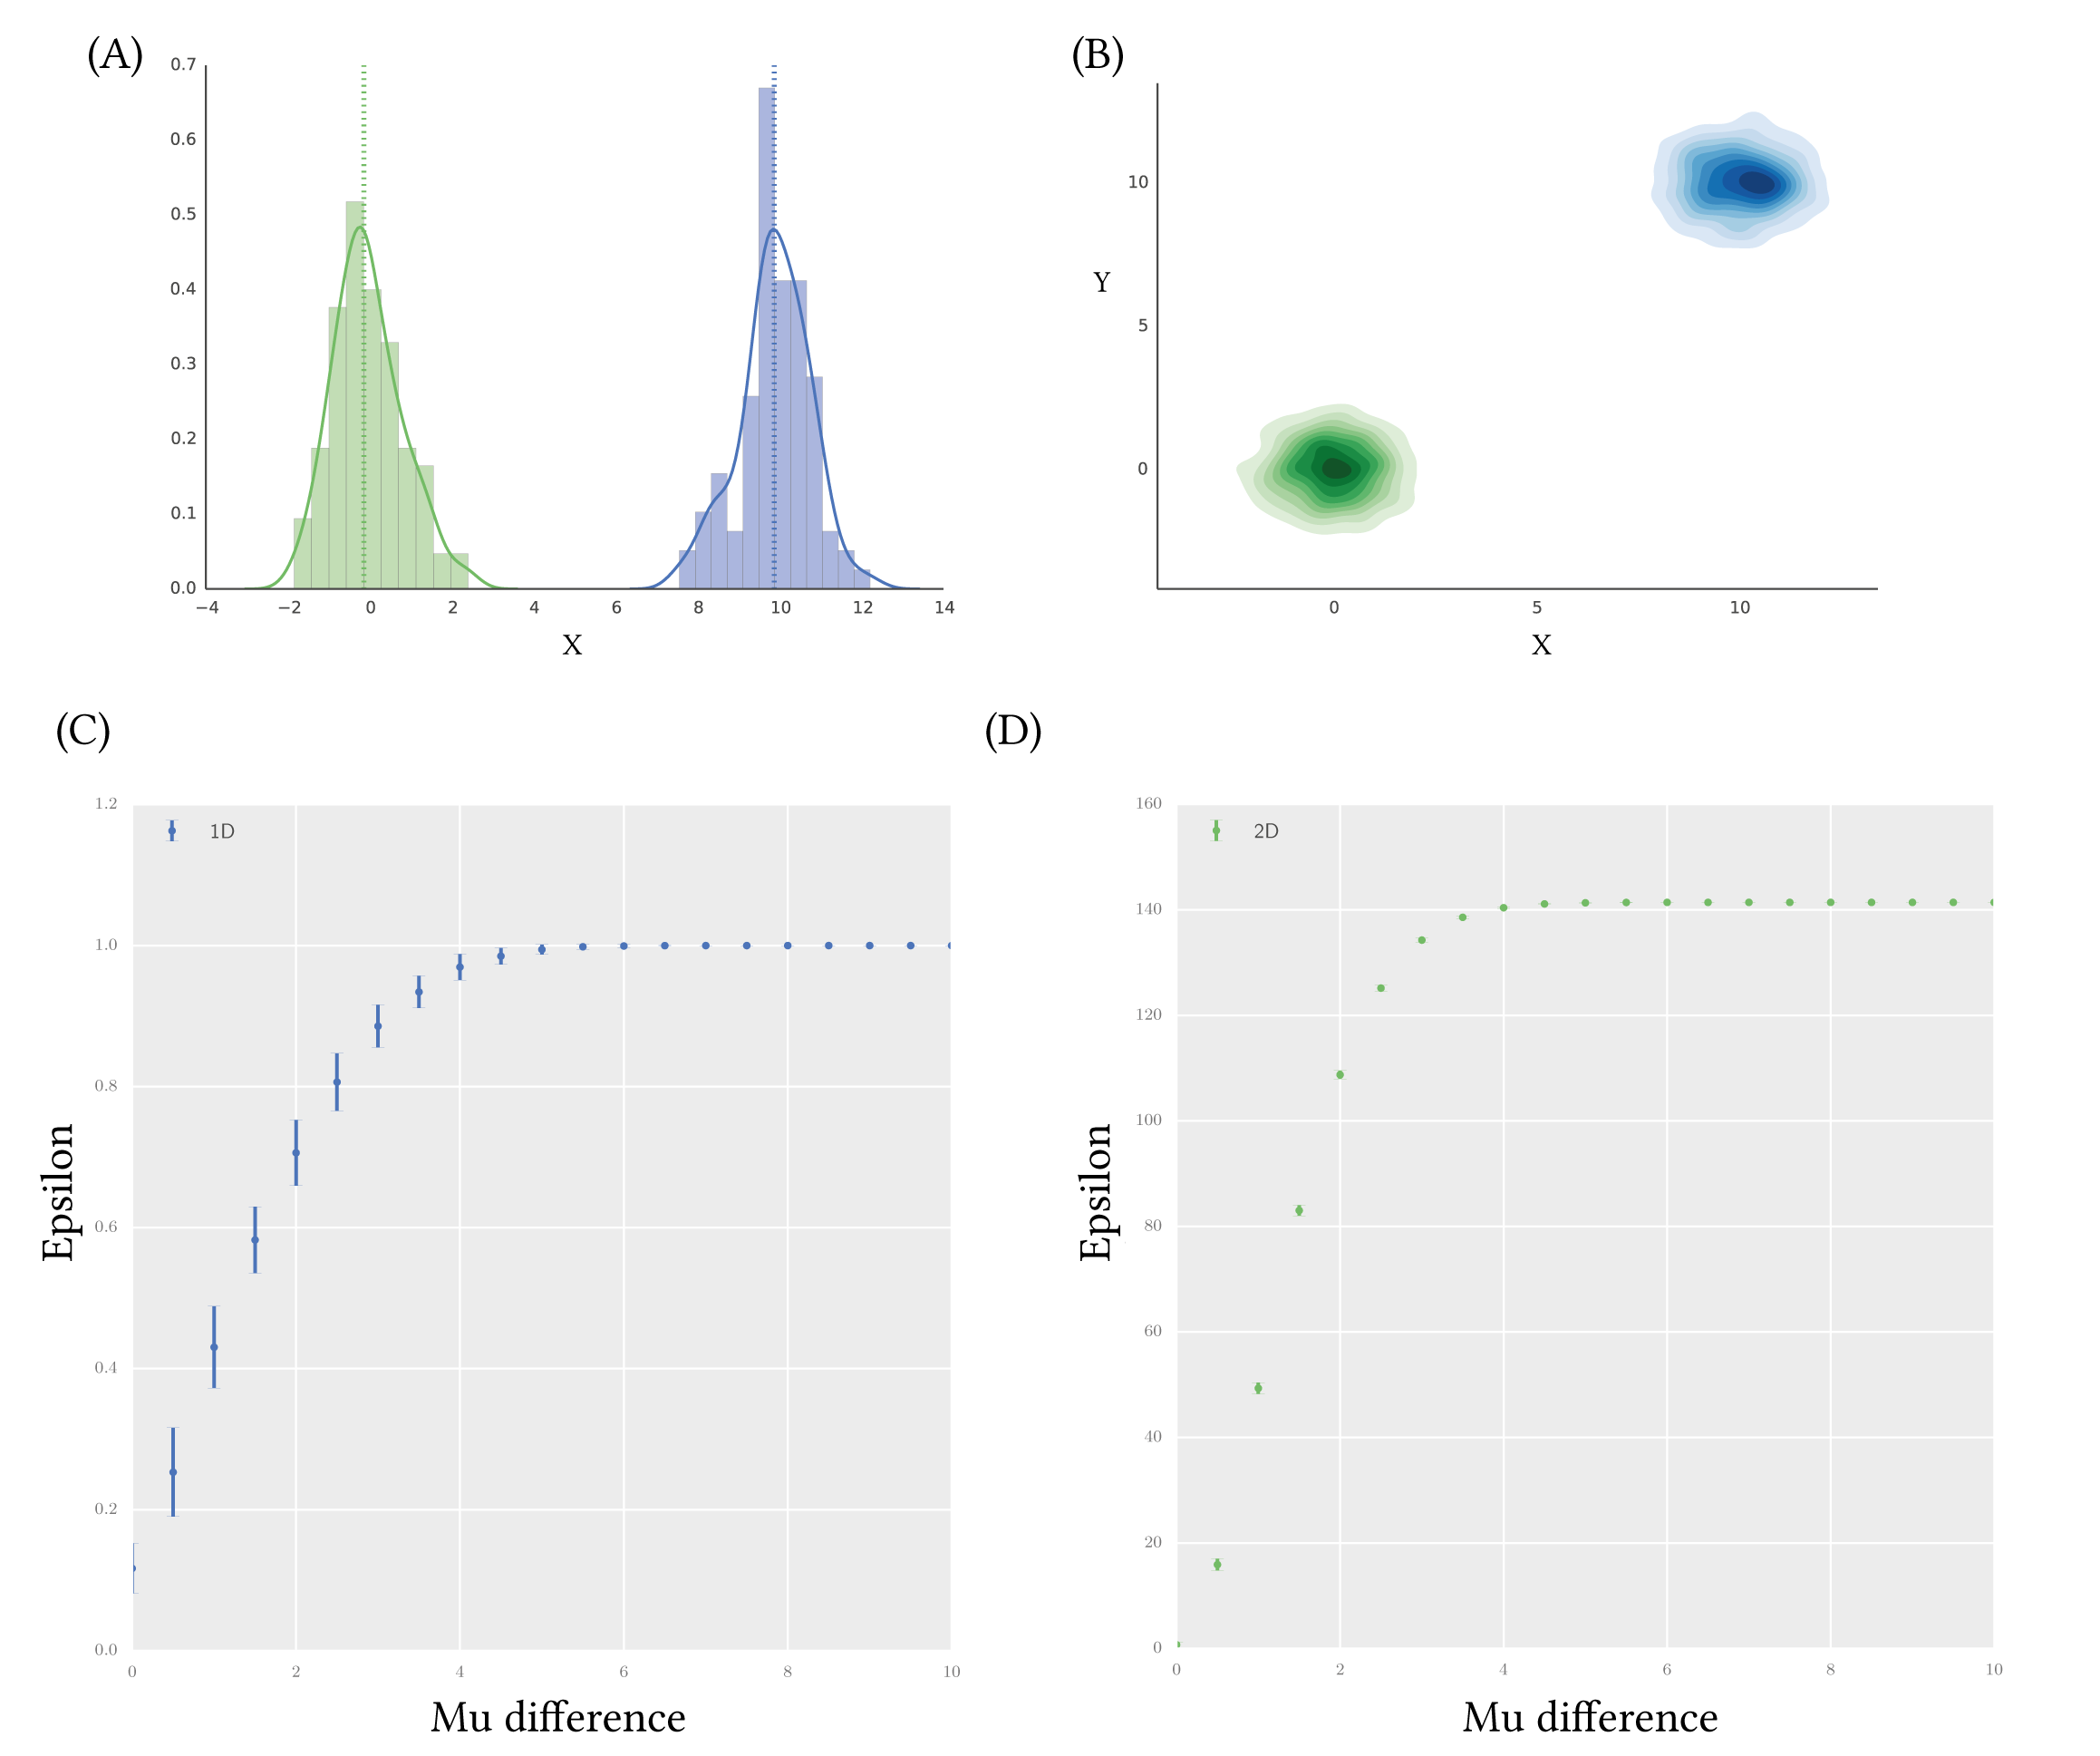
\includegraphics[scale=0.7]{chapterABCFlow/images/mu_diff.png}
\caption[LoF caption]{\label{fig:epsilon_mud} The distance calculation for data sets drawn from increasingly different distributions. Two examples are shown of distributions compared in (A) 1D and (B) 2D. (C) As the difference between the means of the two distributions increases, the distance calculation, epsilon, increases. In the 2D case (shown in green) epsilon plateaus at 2.3 and in the 1D case (shown in blue) epsilon plateaus at 1.}
\label{fig:normal_example}
\end{figure}



%The next parameter to be optimised is the bin size used in the distance calculation. In both 1D and 2D, the space is divided into bins, and the distance between corresponding bins in the data and the simulated data is calculated. The overall distance between to distributions is the sum of the distances between corresponding bins. %If the bin size is too large, small differences between 


%We find that the 2D distance is more sensitive to the bin size than the 1D distance. From Figure~\ref{fig:epsilon_ngrid} we conclude that for a sample size of 100 data points, the optimal bin size for 1D and 2D distance calculation is 10. The above optimizations have been made by using standard normal distributions, of $\mu=0$ and $\sigma=1$. Here we investigate whether the distance calculation depends on the $\mu$ and $sigma$ of the distributions. 

%Next, by varying the amount of $\mu$ and $\sigma$ by which the two normals differ, we can find out the dynamical range of the epsilons. Whether two distributions are identical or vary by a large amount, we can get an estimate of how much the epsilon will vary from one to the other, both in 1D and 2D. 


%From Figure~\ref{fig:epsilon_mu_s_diff} we find that as the difference in $\mu$ increases the epsilon medians reach a plateau. We find that beyond a difference of 4 in $\mu$, the distance calculation cannot further separate the distances. This can be caused by the fact that when first dividing the space into bins, the range of the data is used to define the grid. If all the simulated data is located outside that grid, the algorithm can no longer distinguish between them, and will only allocate them as outside the range. The variance of the epsilon distributions does not vary significantly with increasing difference in $\mu$. As the difference in $\sigma$ increases between the distributions, we find that the median in the 2D distance calculation increases but not in the 1D. Note, that the range of the difference in the epsilon medians is small and thus we conclude that differences in the $\mu$ of a distribution are much better detected than the differences in the $\sigma$. The variance of the epsilon distribution when $\sigma$ is varied does not change significantly with increasing $\sigma$ difference.


%We study the epsilon distribution variance in the uniform distribution, [0, 1].  
%When comparing a normally distributed data set to a uniformly distributed data set, we don't see a great difference between the 1D and 2D epsilons.


%Another type of distribution that is commonly found in Flow cytometry experiments, is a bimodal distribution. Here we test whether the 1D and 2D distances are equivalent when measuring distances in this type of distributions.


%Finally, we study how the distances perform when comparing a bimodal with a normal distribution. We test the distances by using a bimodal distribution and a series of normal distributions with increasing $\mu$, in 1D and 2D. We find that epsilon is the lowest when the $\mu$ of the normal distribution corresponds to the $\mu$ of one of the two peaks in the bimodal distribution and the highest when there is no overlap between the distributions. 



\clearpage
\subsubsection{ABC-Flow validation using simulated data}

In this section I apply ABC-Flow to simulated data, where the parameter values used to produce the data are known. This analysis will serve as a verification test for ABC-Flow. The model used to produce the simulated data is an extension of the~\textcite{Gardner:2000vha} switch. The model consists of two mutually repressing transcription factors. The model used here has additional parameters, representing the repression from the external repressors, \acrshort{iptg} and \acrshort{atc}. 

In order to produce the simulated data set, the extended~\textcite{Gardner:2000vha} switch was simulated stochastically using the Gillespie algorithm~\autocite{Gillespie:1977ww}. The model used is defined by the following hazards:

\begin{align}
h_1 &= u \label{eq:eg1}\\
h_2 &= \frac{p_1 \times p_3	}{1+p_3+v^{p_2}} \label{eq:eg2}\\
h_3 &= (1 + a)\times v \label{eq:eg3}\\
h_4 &= \frac{p_4\times p_6}{1+p_6+u^{p_5}} \label{eq:eg4}
\end{align}


Using the time course data generated for one of the fluorescent proteins in the system, $u$, I use ABC-Flow to fit the model shown above, using priors centered around the parameter values used to produce the data. The resulting fit is shown in Figure~\ref{fig:1d-sim-res}A. In order to determine whether this is a good fit to the data, QQ plots are produced for each timepoint (Figure~\ref{fig:1d-sim-res}B). A QQ-plot is a plot where the quantiles of two distributions are plotted against eachother. If the distributions are similar, the points will lie on the 45\textdegree{} line x = y line~\autocite{Wilk:1968ts}. 


\begin{figure}[htbp]
\centering
	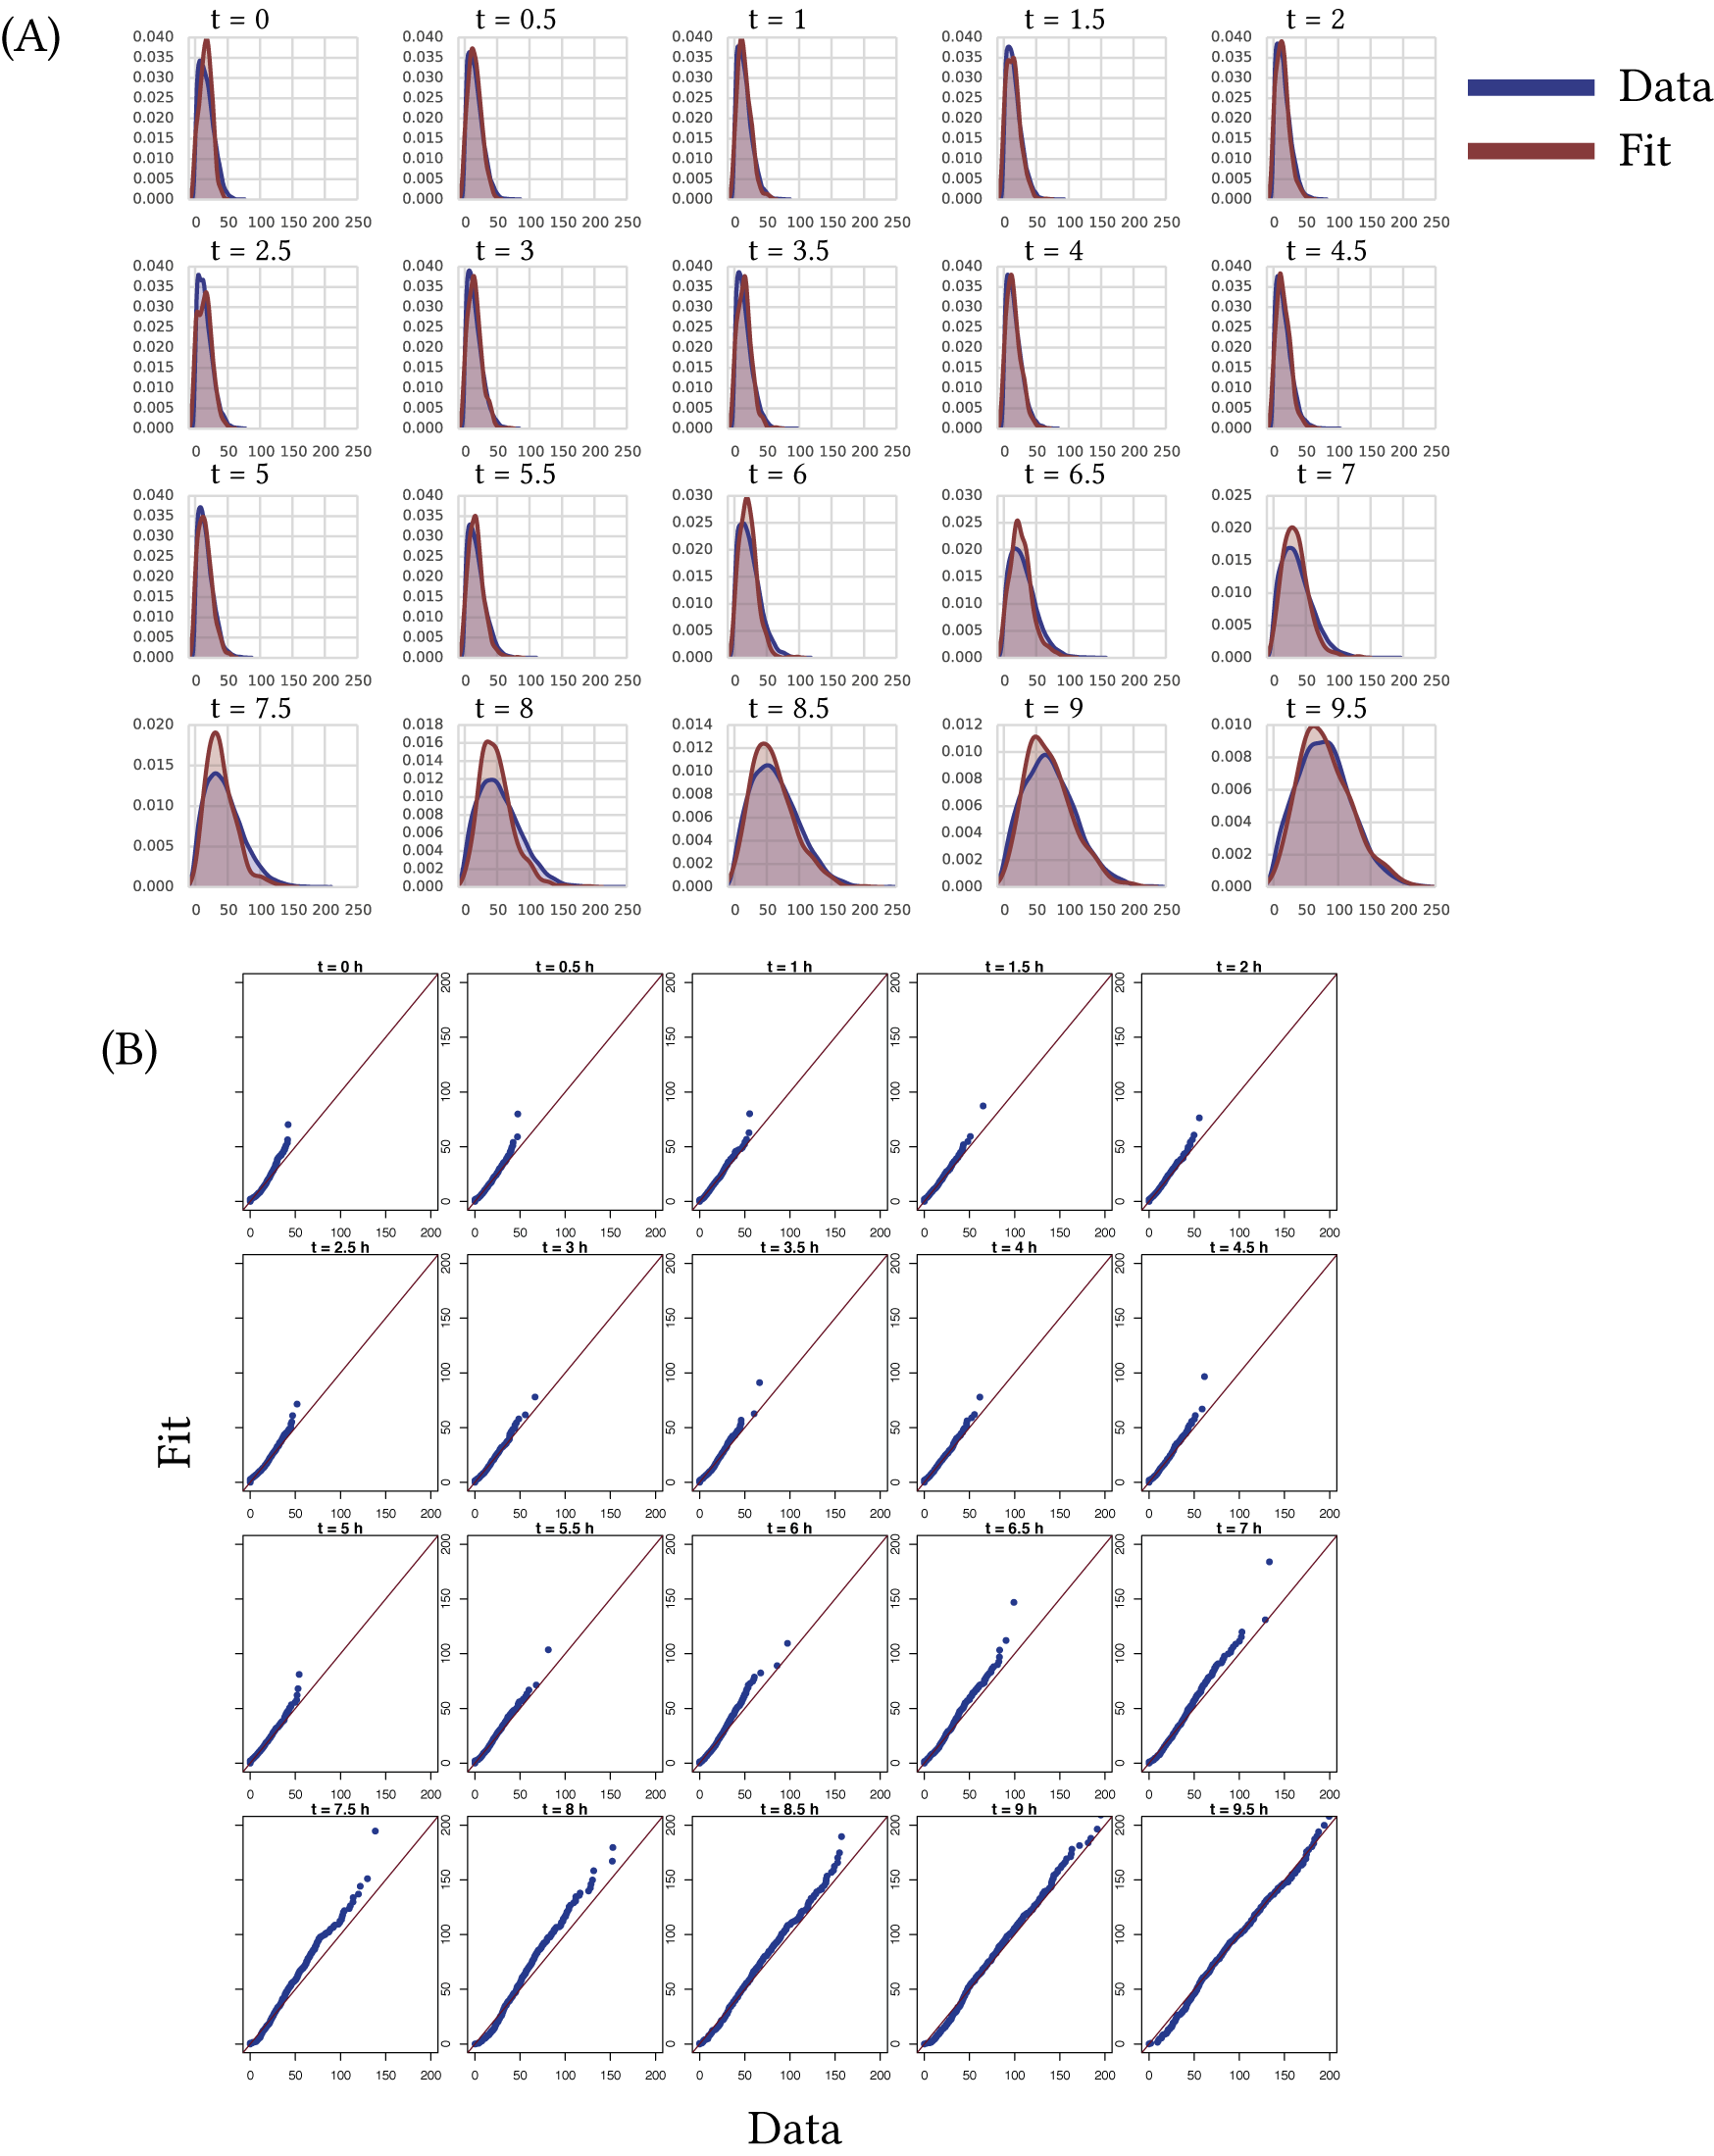
\includegraphics[scale=0.8]{chapterABCFlow/images/1D_sim_res.png}
	\caption[LoF caption]{\label{fig:1d-sim-res} (A) 1D ABC-Flow fit (shown in blue) to data (shown in red) produced by simulating the same model. (B) QQ-plot of each time point fit. The quantile of the two distributions are plotted against eachother. If the ditributions are similar, the points would lie on the 45\textdegree{} line x = y, shown in red. }
\end{figure}
\clearpage

By examining the data and the fitted models shown in Figure~\ref{fig:1d-sim-res}, we see that at \textepsilon = 0.1, there is a good fit of the model to the data using ABC-Flow. The model parameters, as well as the intensity parameters, have been fitted to simulated flow cytometry data. The timecourse of the model after fitting with ABC-Flow is similar to the data time course. 

I further test ABC-Flow by using 2D data to fit two species of the model simultaneously. The same data was used as was used in the 1D case, but this time both species $u$ and $v$ were taken into account. This represents both sides of the switch model used. Using the same priors as in the 1D case, we can compare the two fits and investigate whether using the 1D or 2D data results in a better fit. The 1D data represents one of the marginal distributions of the data sets, as illustrated in Figure~\ref{fig:1d2dsketch}. I use the marginal distribution of $u$ and the bivariate distribution of $u$ and $v$ in order to determine which one produces a better fit to the data. The resulting timecourse of the data as well as the 1D and 2D fit are shown in Figure~\ref{fig:1d2dcomp}.


\begin{figure}[htbp]
\centering
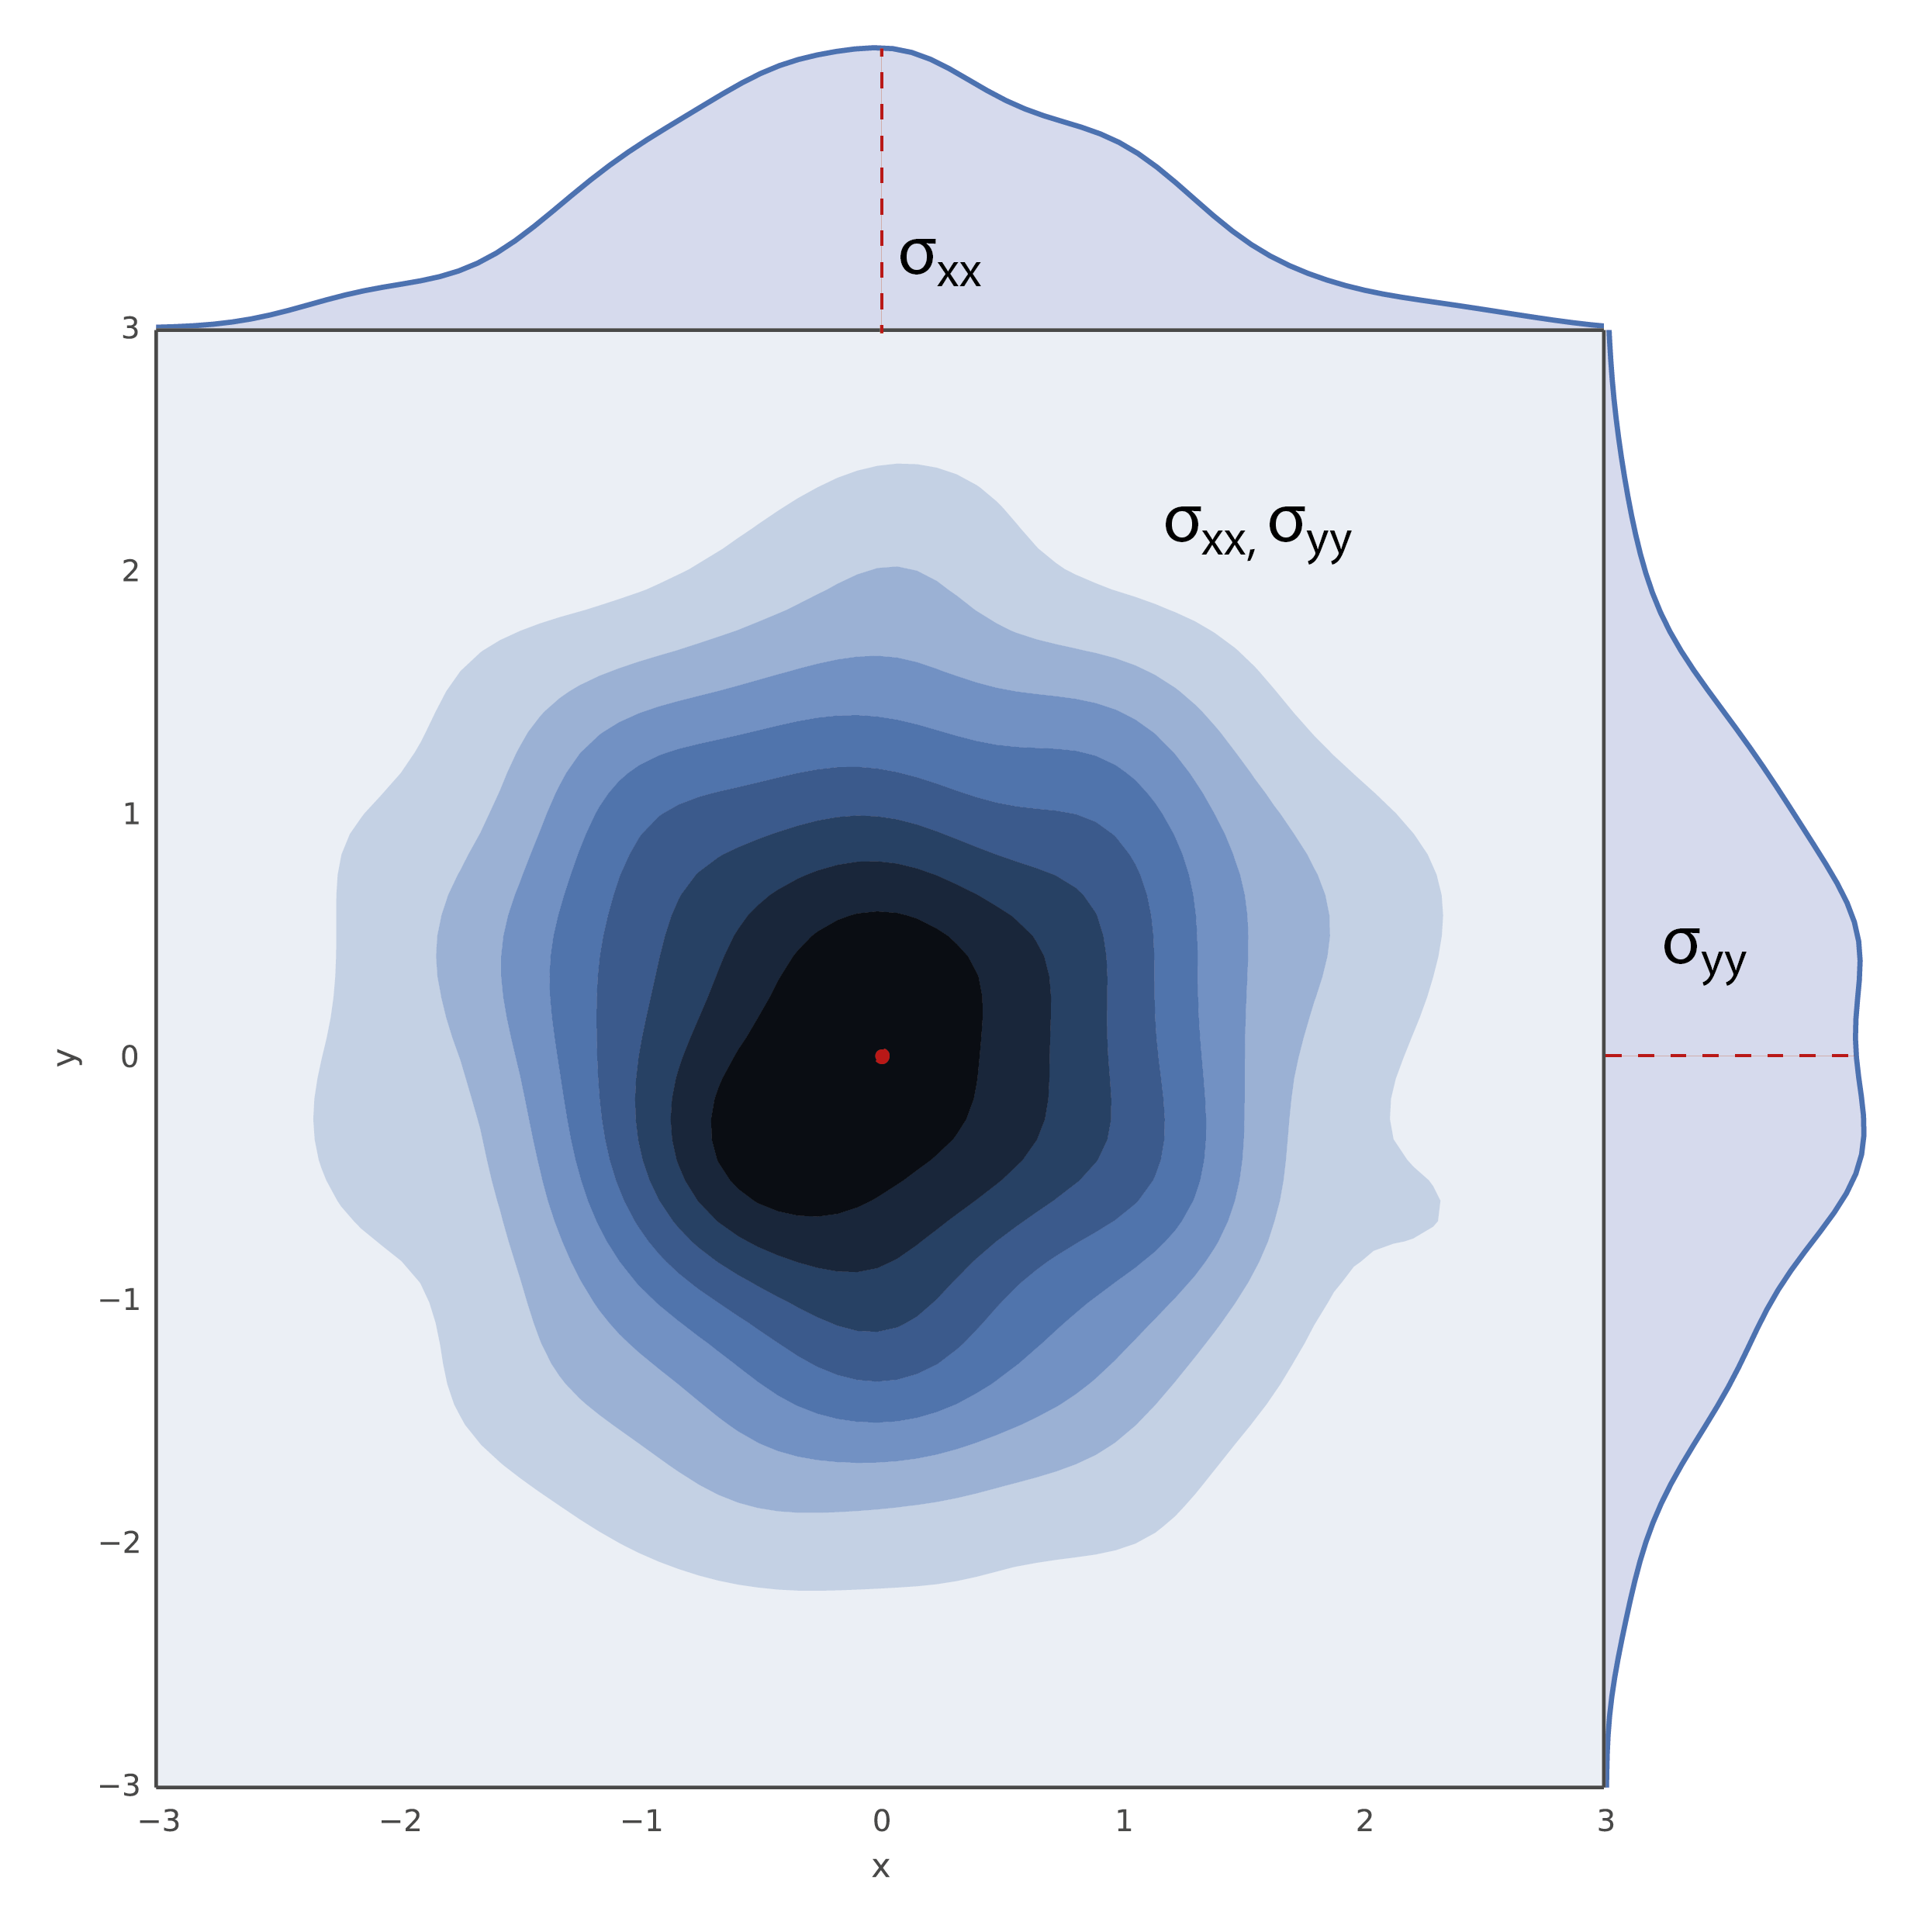
\includegraphics[scale=0.3]{chapterABCFlow/images/normal_sigma_example.png}
\caption[LoF caption]{\label{fig:1d2dsketch} The marginal (1D) versus the bivariate (2D) distribution of the data.}
\end{figure}




\begin{figure}[htbp]
\centering
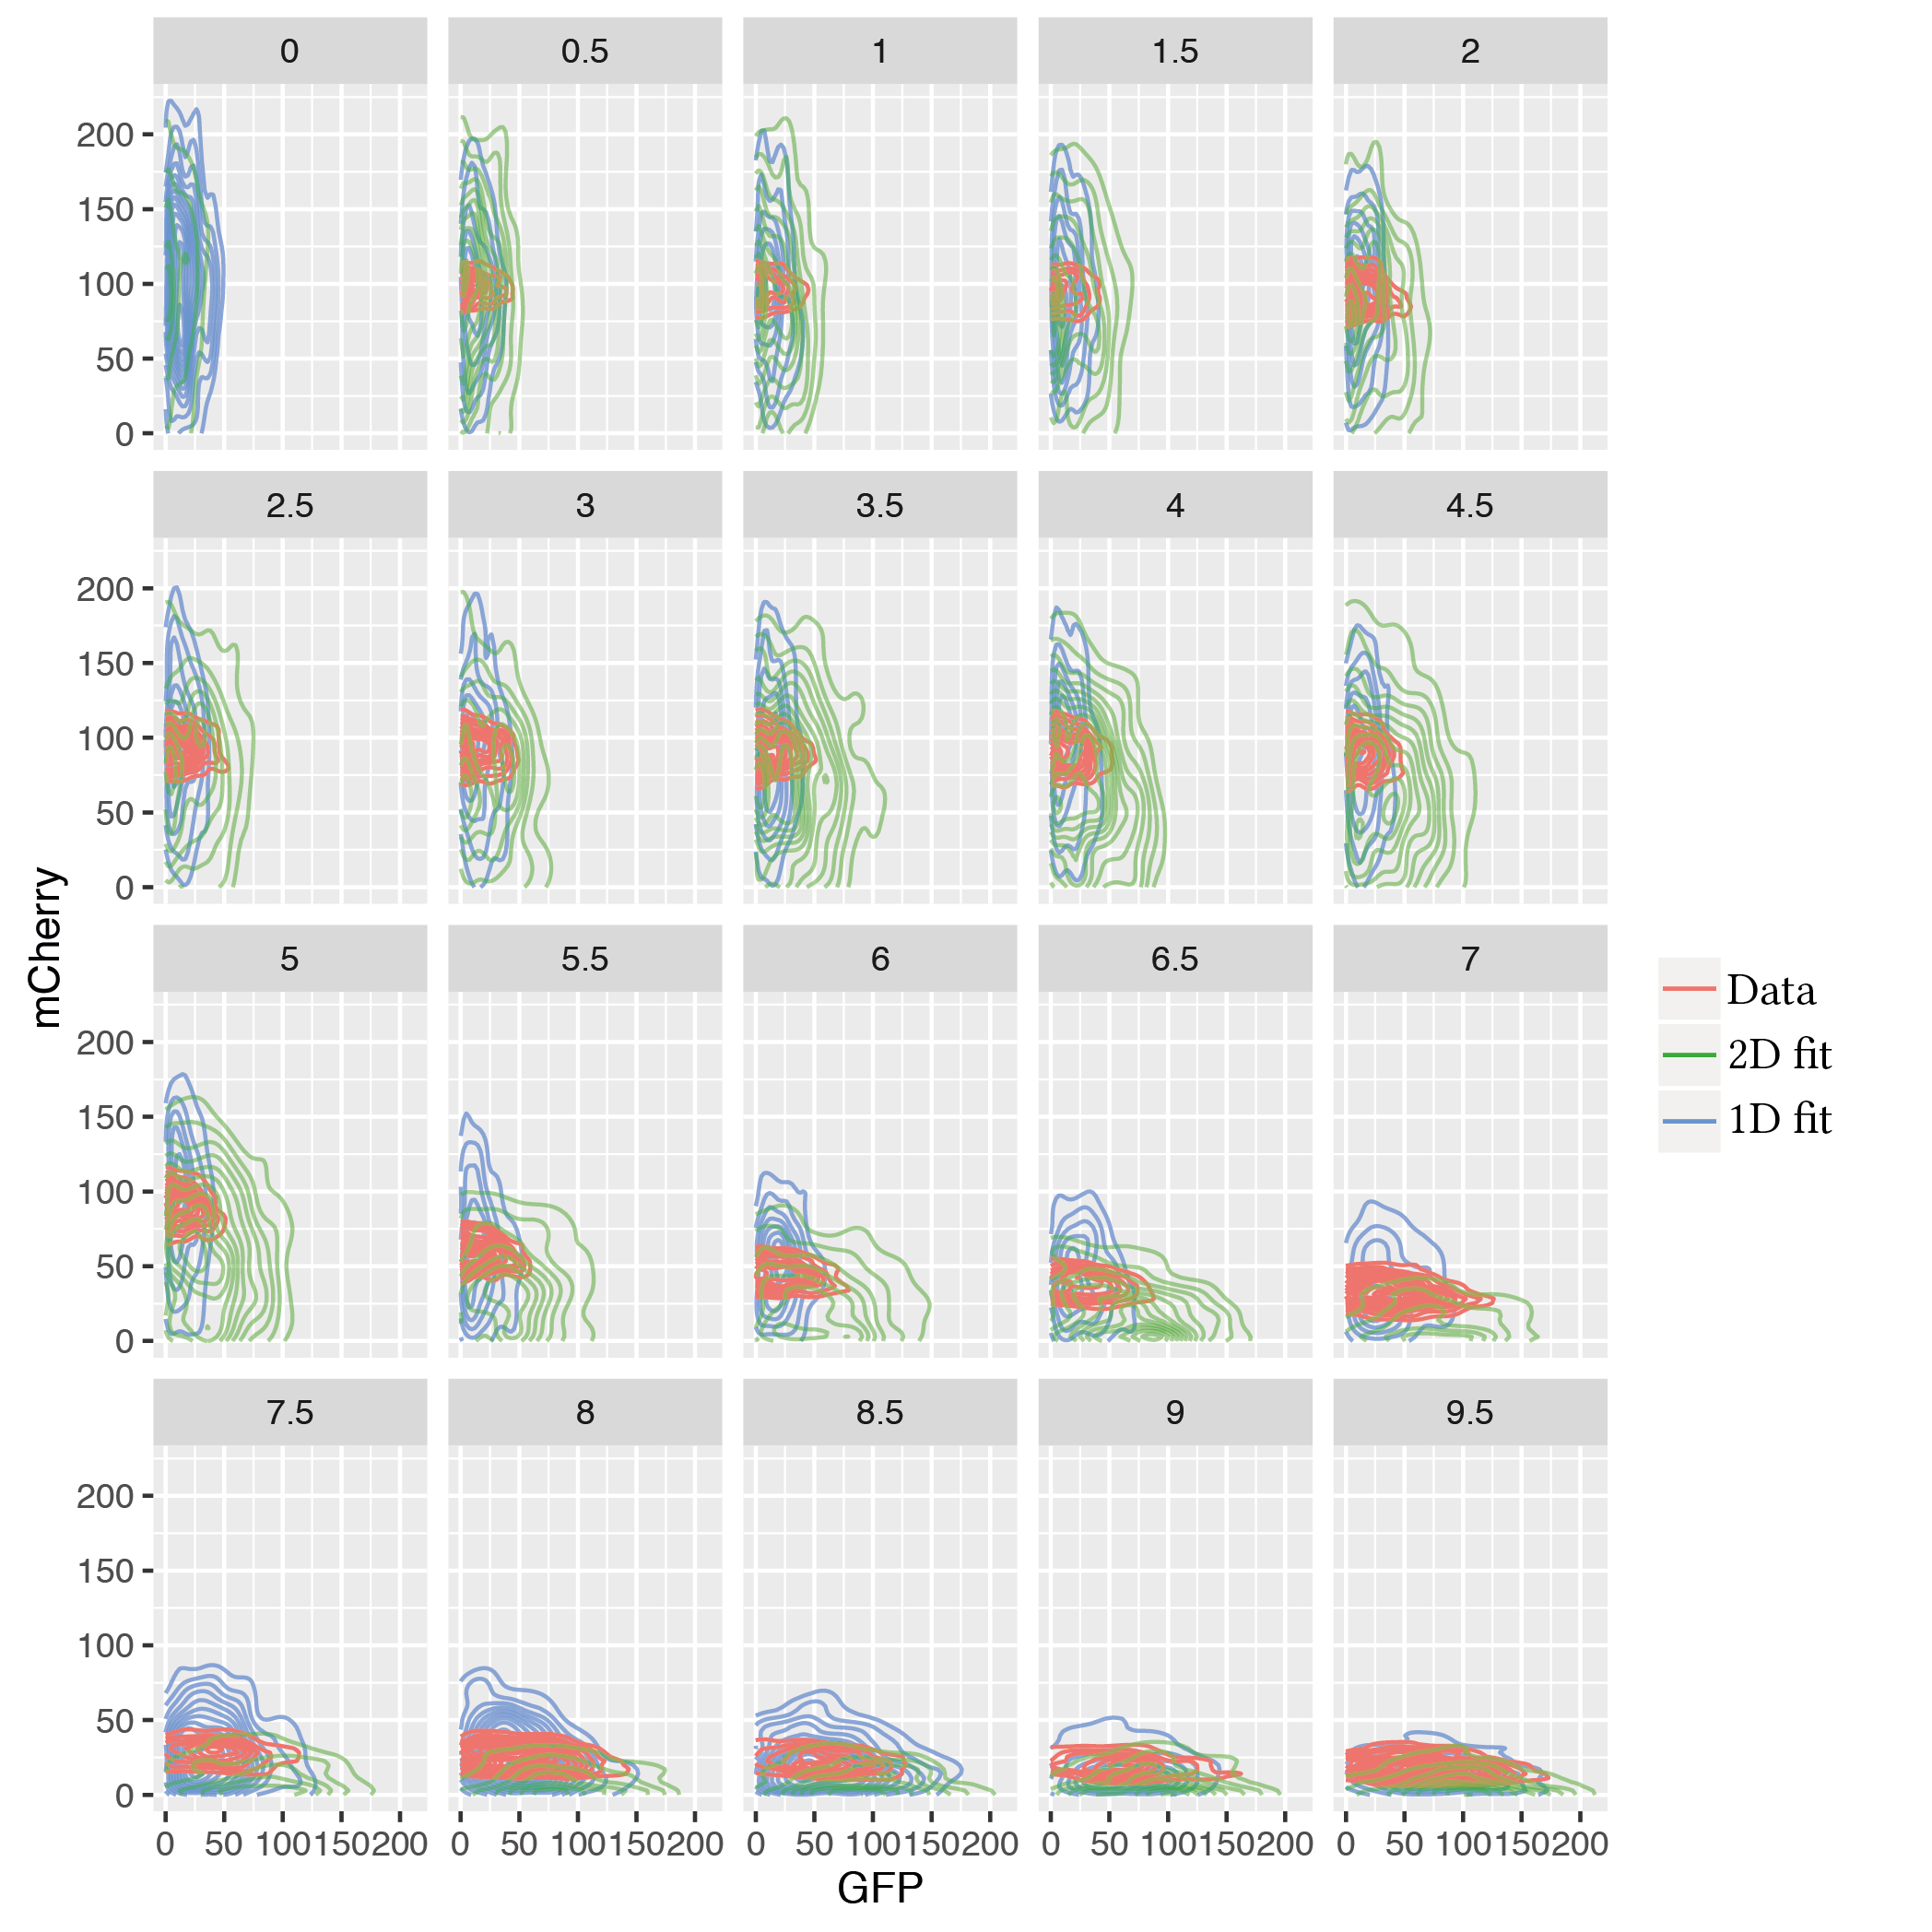
\includegraphics[scale=0.8]{chapterABCFlow/images/compare_1D_2d.png}
\caption[LoF caption]{\label{fig:1d2dcomp} Comparing the fits obtained by using the 1D or 2D data. }
\end{figure}
\clearpage


The posterior distributions obtained from each fit are shown in Figure~\ref{fig:1d2d-sim-post}. We find similar posterior ranges for both the 1D and 2D fits.

\begin{figure}[htbp]
\centering
	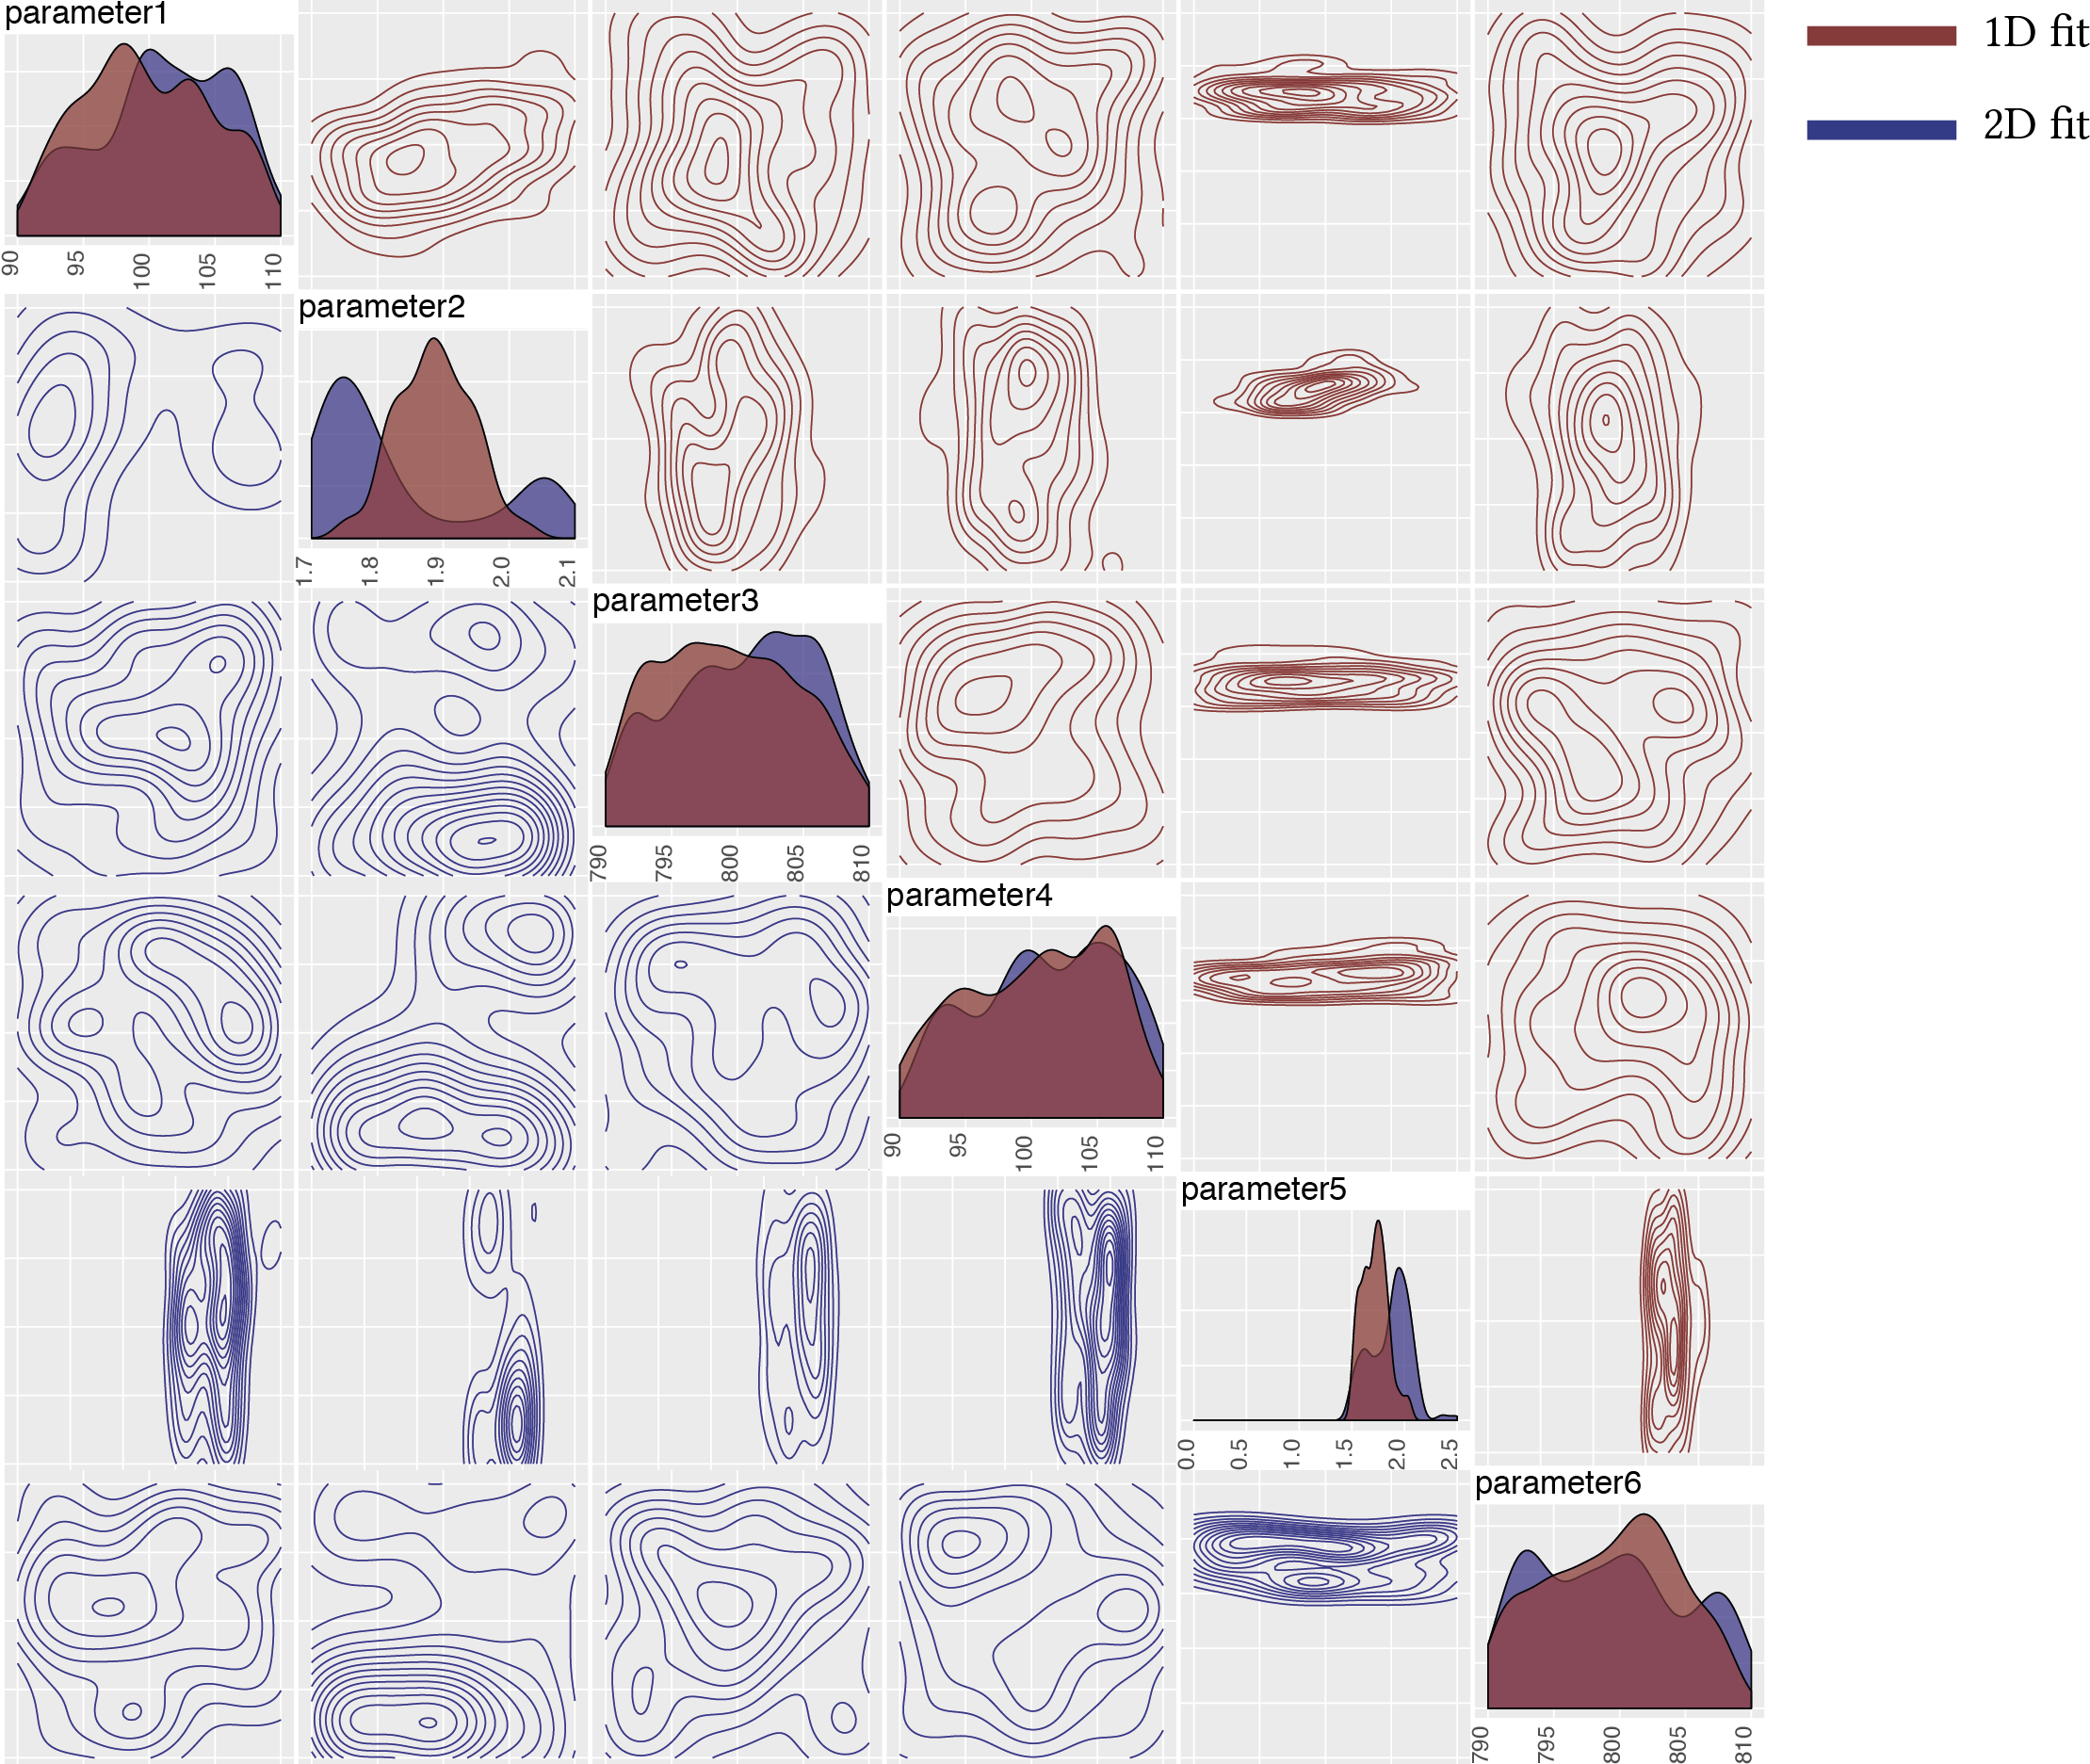
\includegraphics[scale=0.8]{chapterABCFlow/images/sim_1d_2d_post.png}
	\caption[LoF caption]{\label{fig:1d2d-sim-post} 1D (red) 2D (blue) fit. }
\end{figure}

%\begin{figure}[htbp]
%\centering%
%	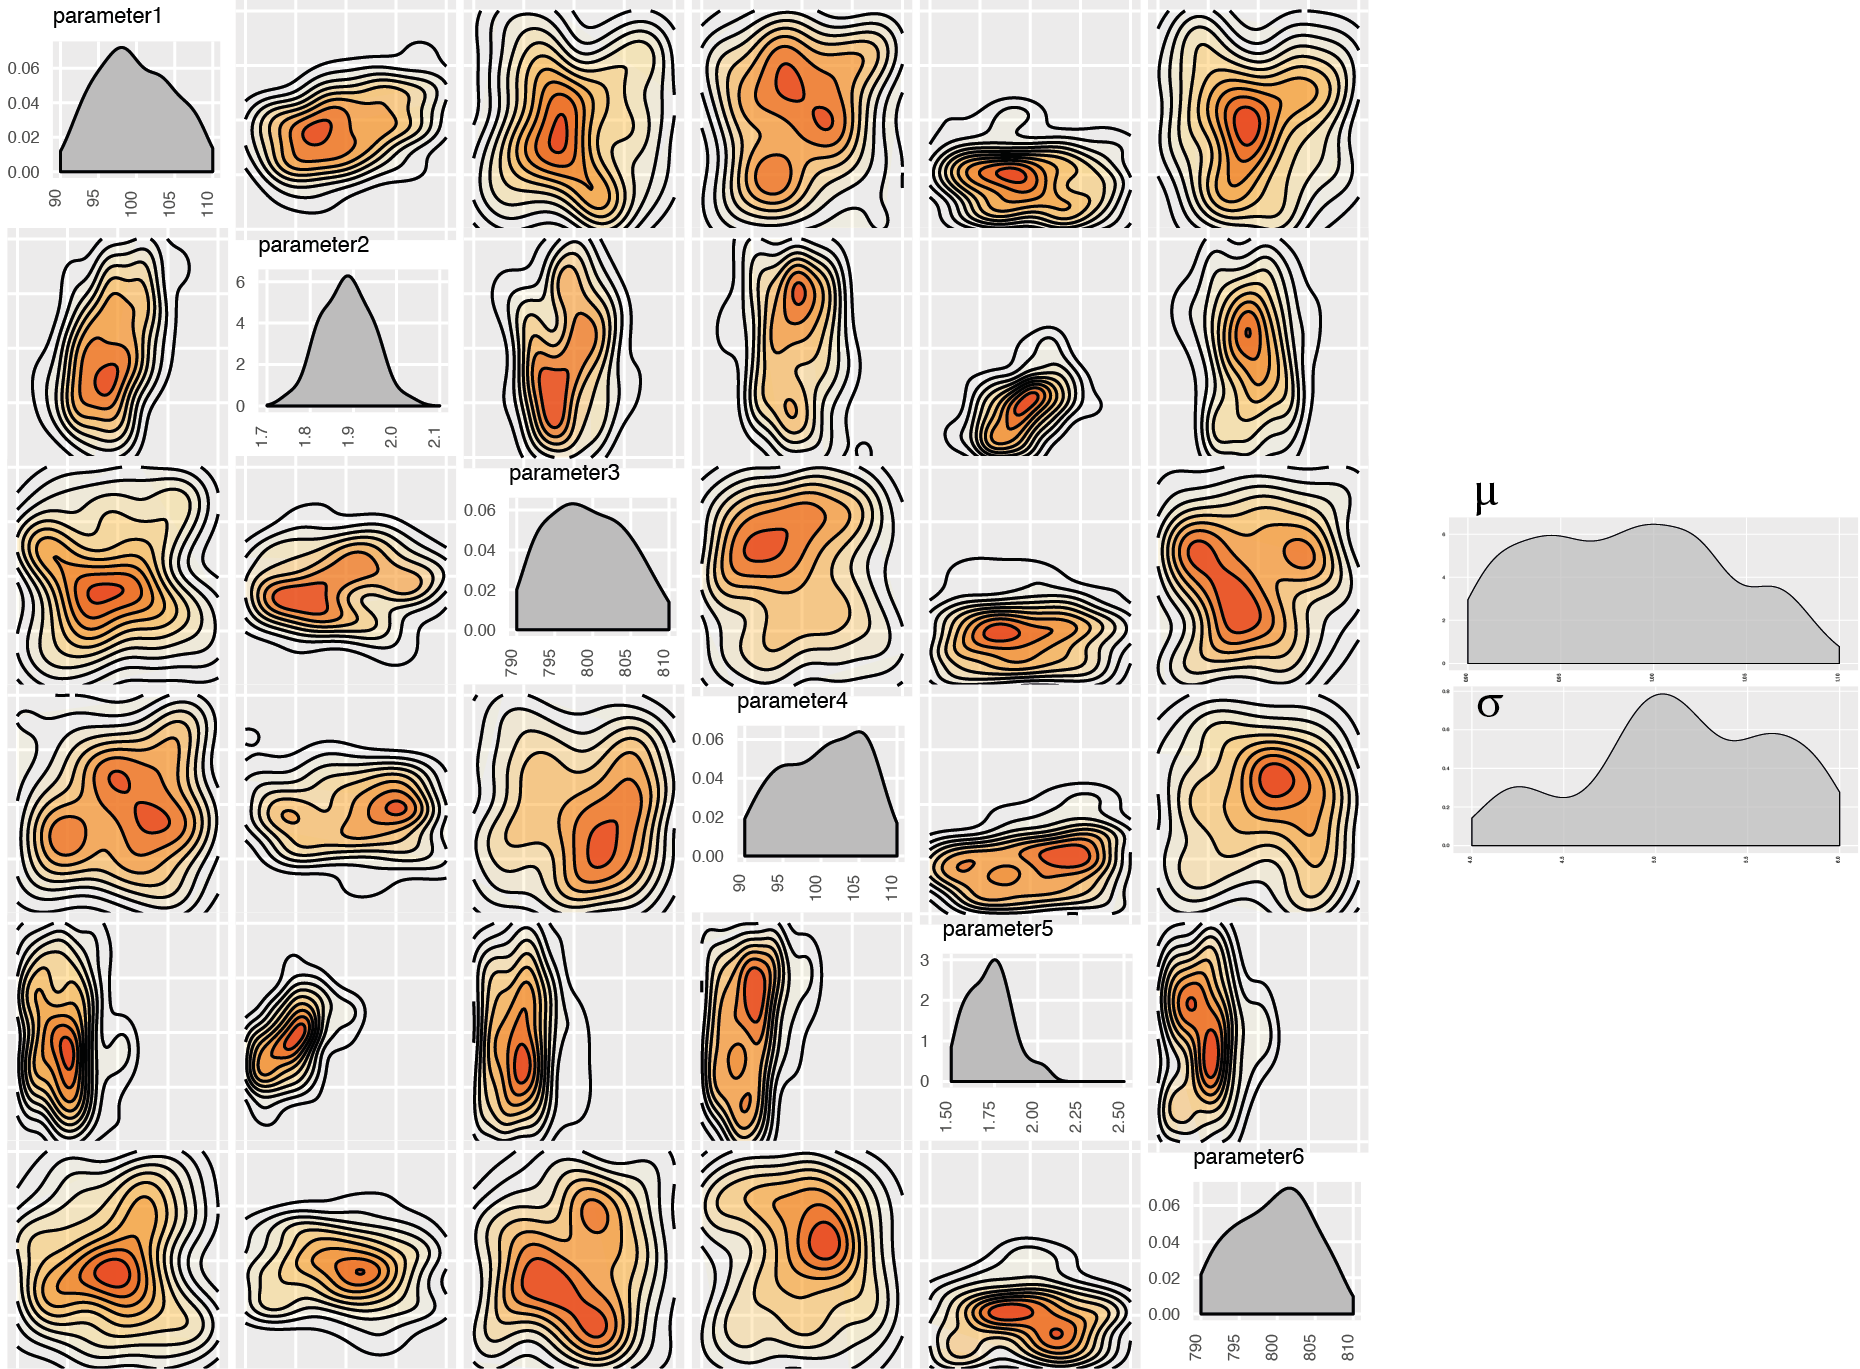
\includegraphics[scale=0.6]{chapterABCFlow/images/1d_sim_post.png}%
%	\caption[LoF caption]{\label{fig:1d-sim-post}}
%\end{figure}



%\begin{figure}[htbp]
%\centering
%	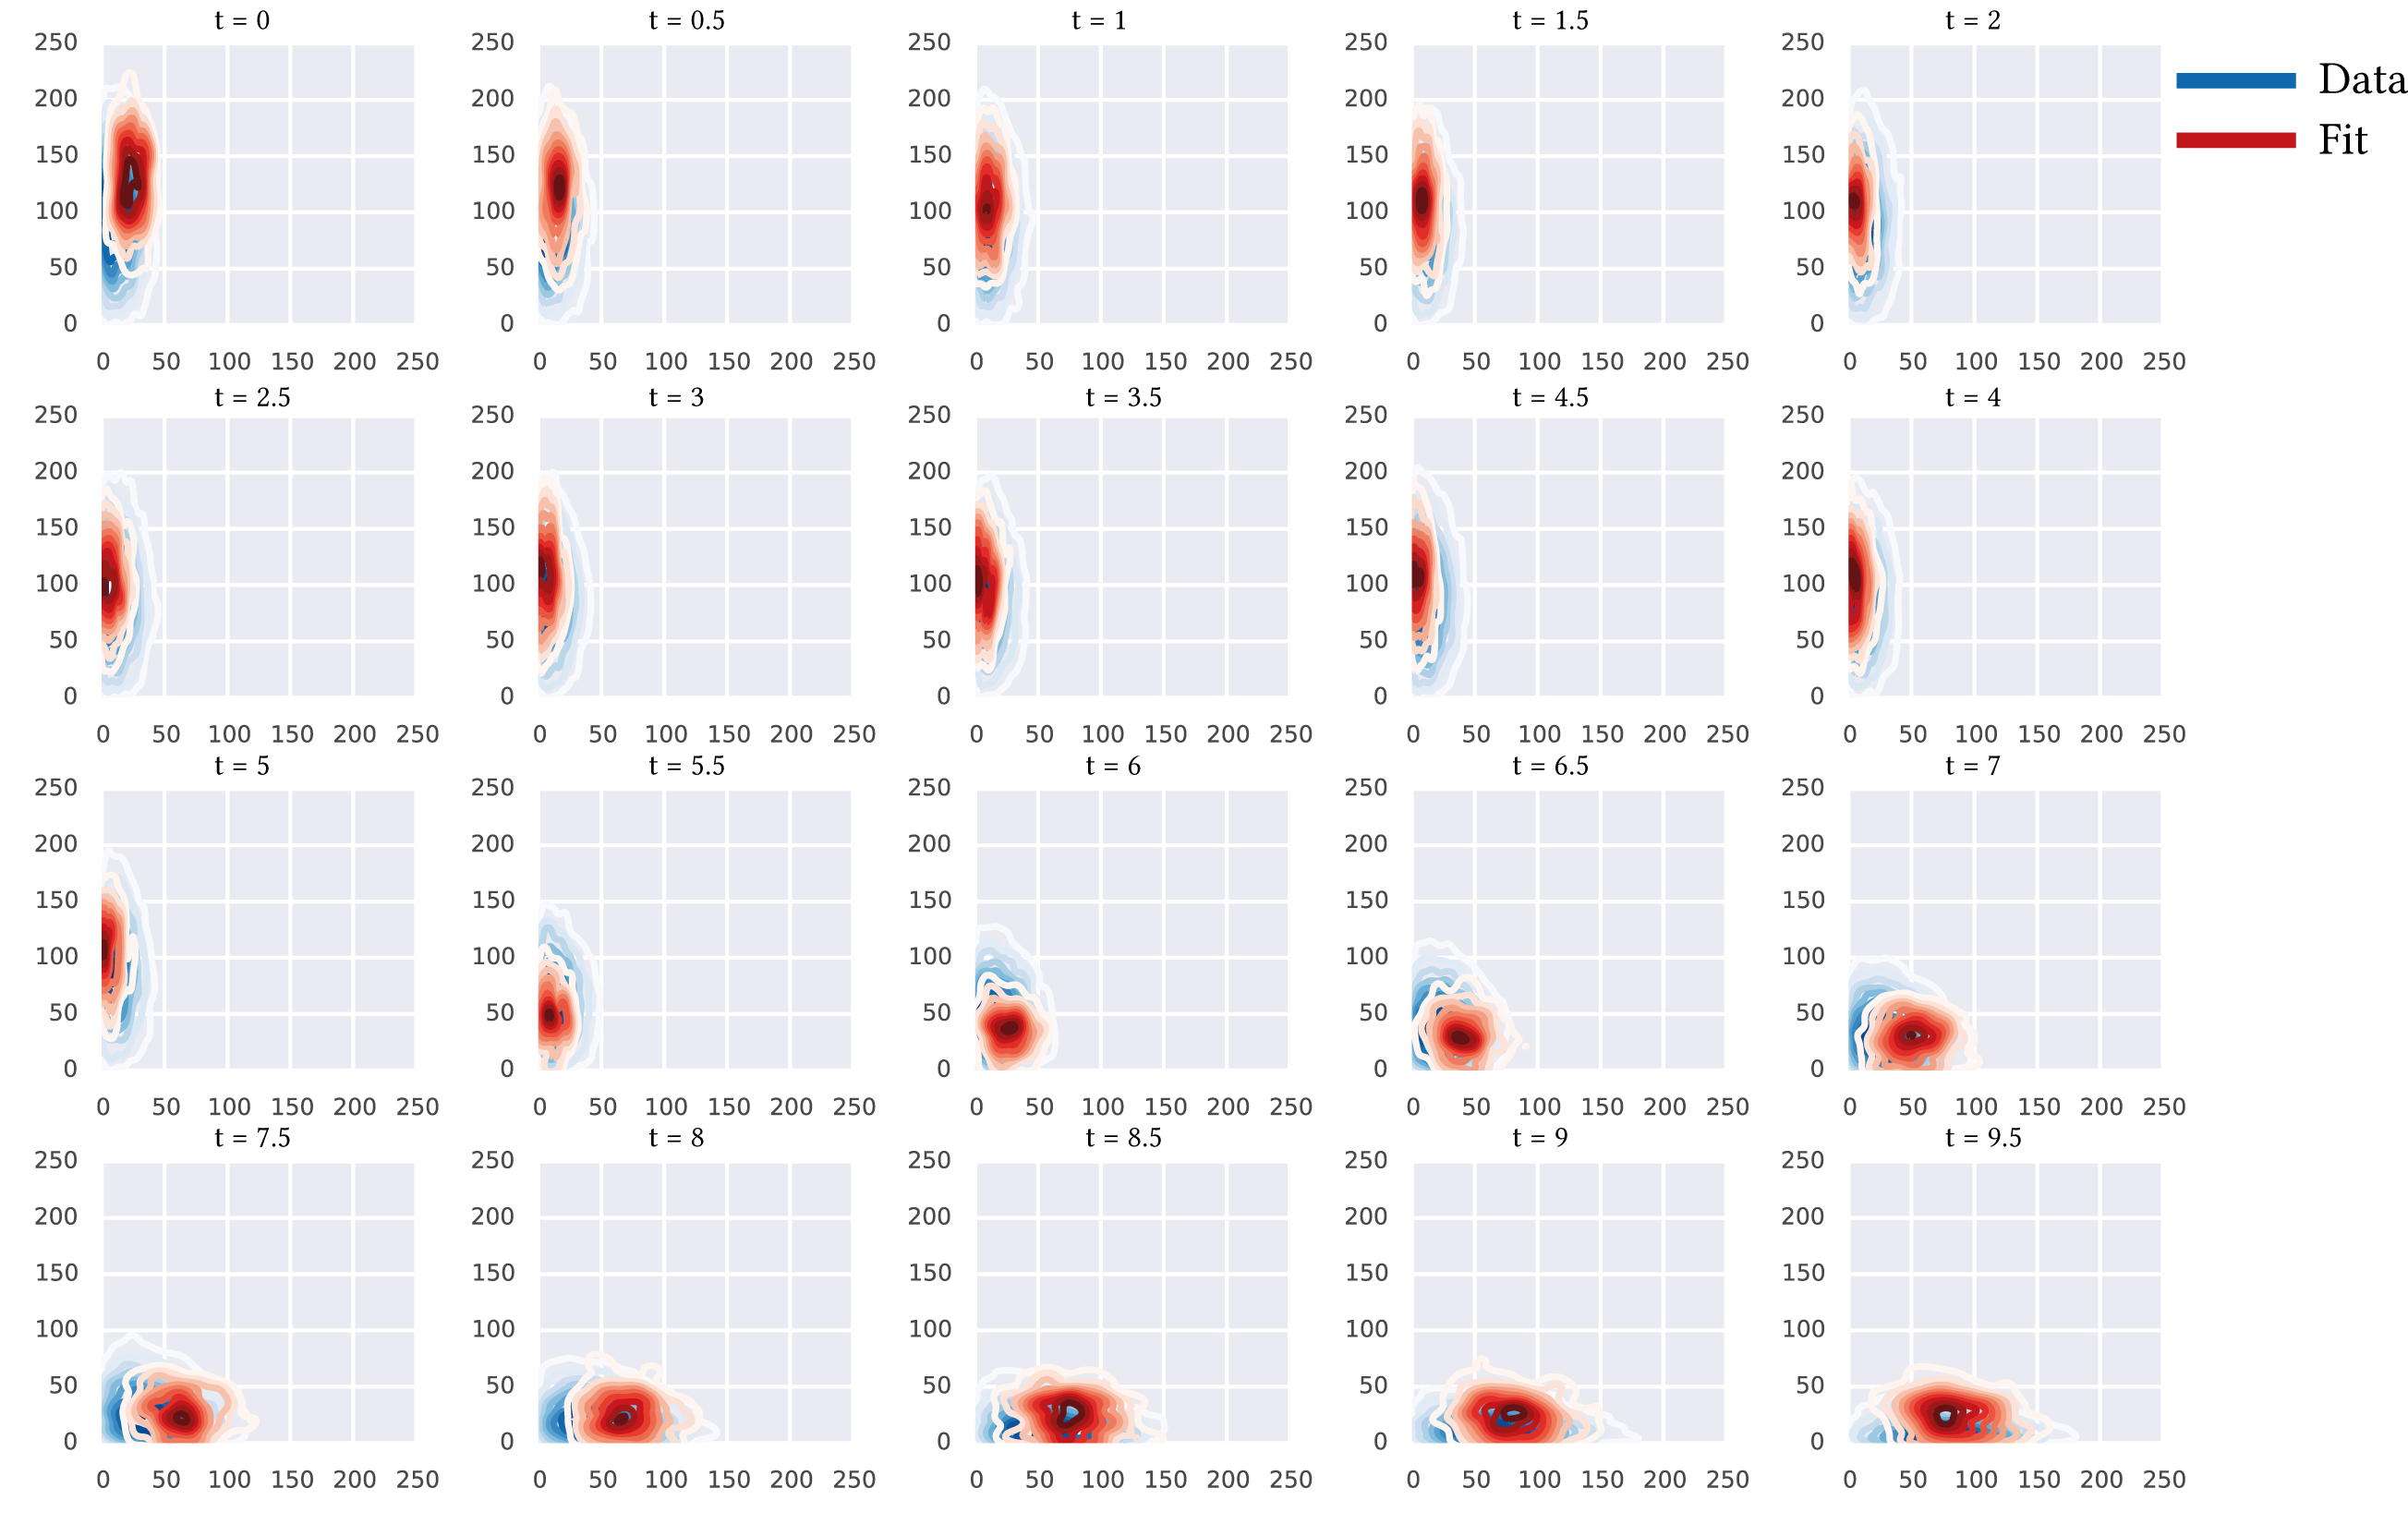
\includegraphics[scale=0.6]{chapterABCFlow/images/2D_sim_res.png}
%	\caption[LoF caption]{\label{fig:2d-sim-res}}
%\end{figure}

\clearpage
\subsubsection{ABC-Flow used on experimental data}
 
Next I applied ABC-Flow to the experimental flow cytometry data collected in Section~\ref{sec:ts_time}. The data set is comprised of time course data of the~\textcite{Litcofsky:2012gr} toggle switch. The two states of the switch are represented by the levels of GFP and mCherry intensity in each bacterial cell. Using \acrshort{atc} inducer, each cell transitions from a mCherry high state to a GFP high state. I used the extension to the~\textcite{Gardner:2000vha} switch described in Equations~\ref{eq:eg1}-\ref{eq:eg4}.

 
\begin{figure}[htbp]
\centering
	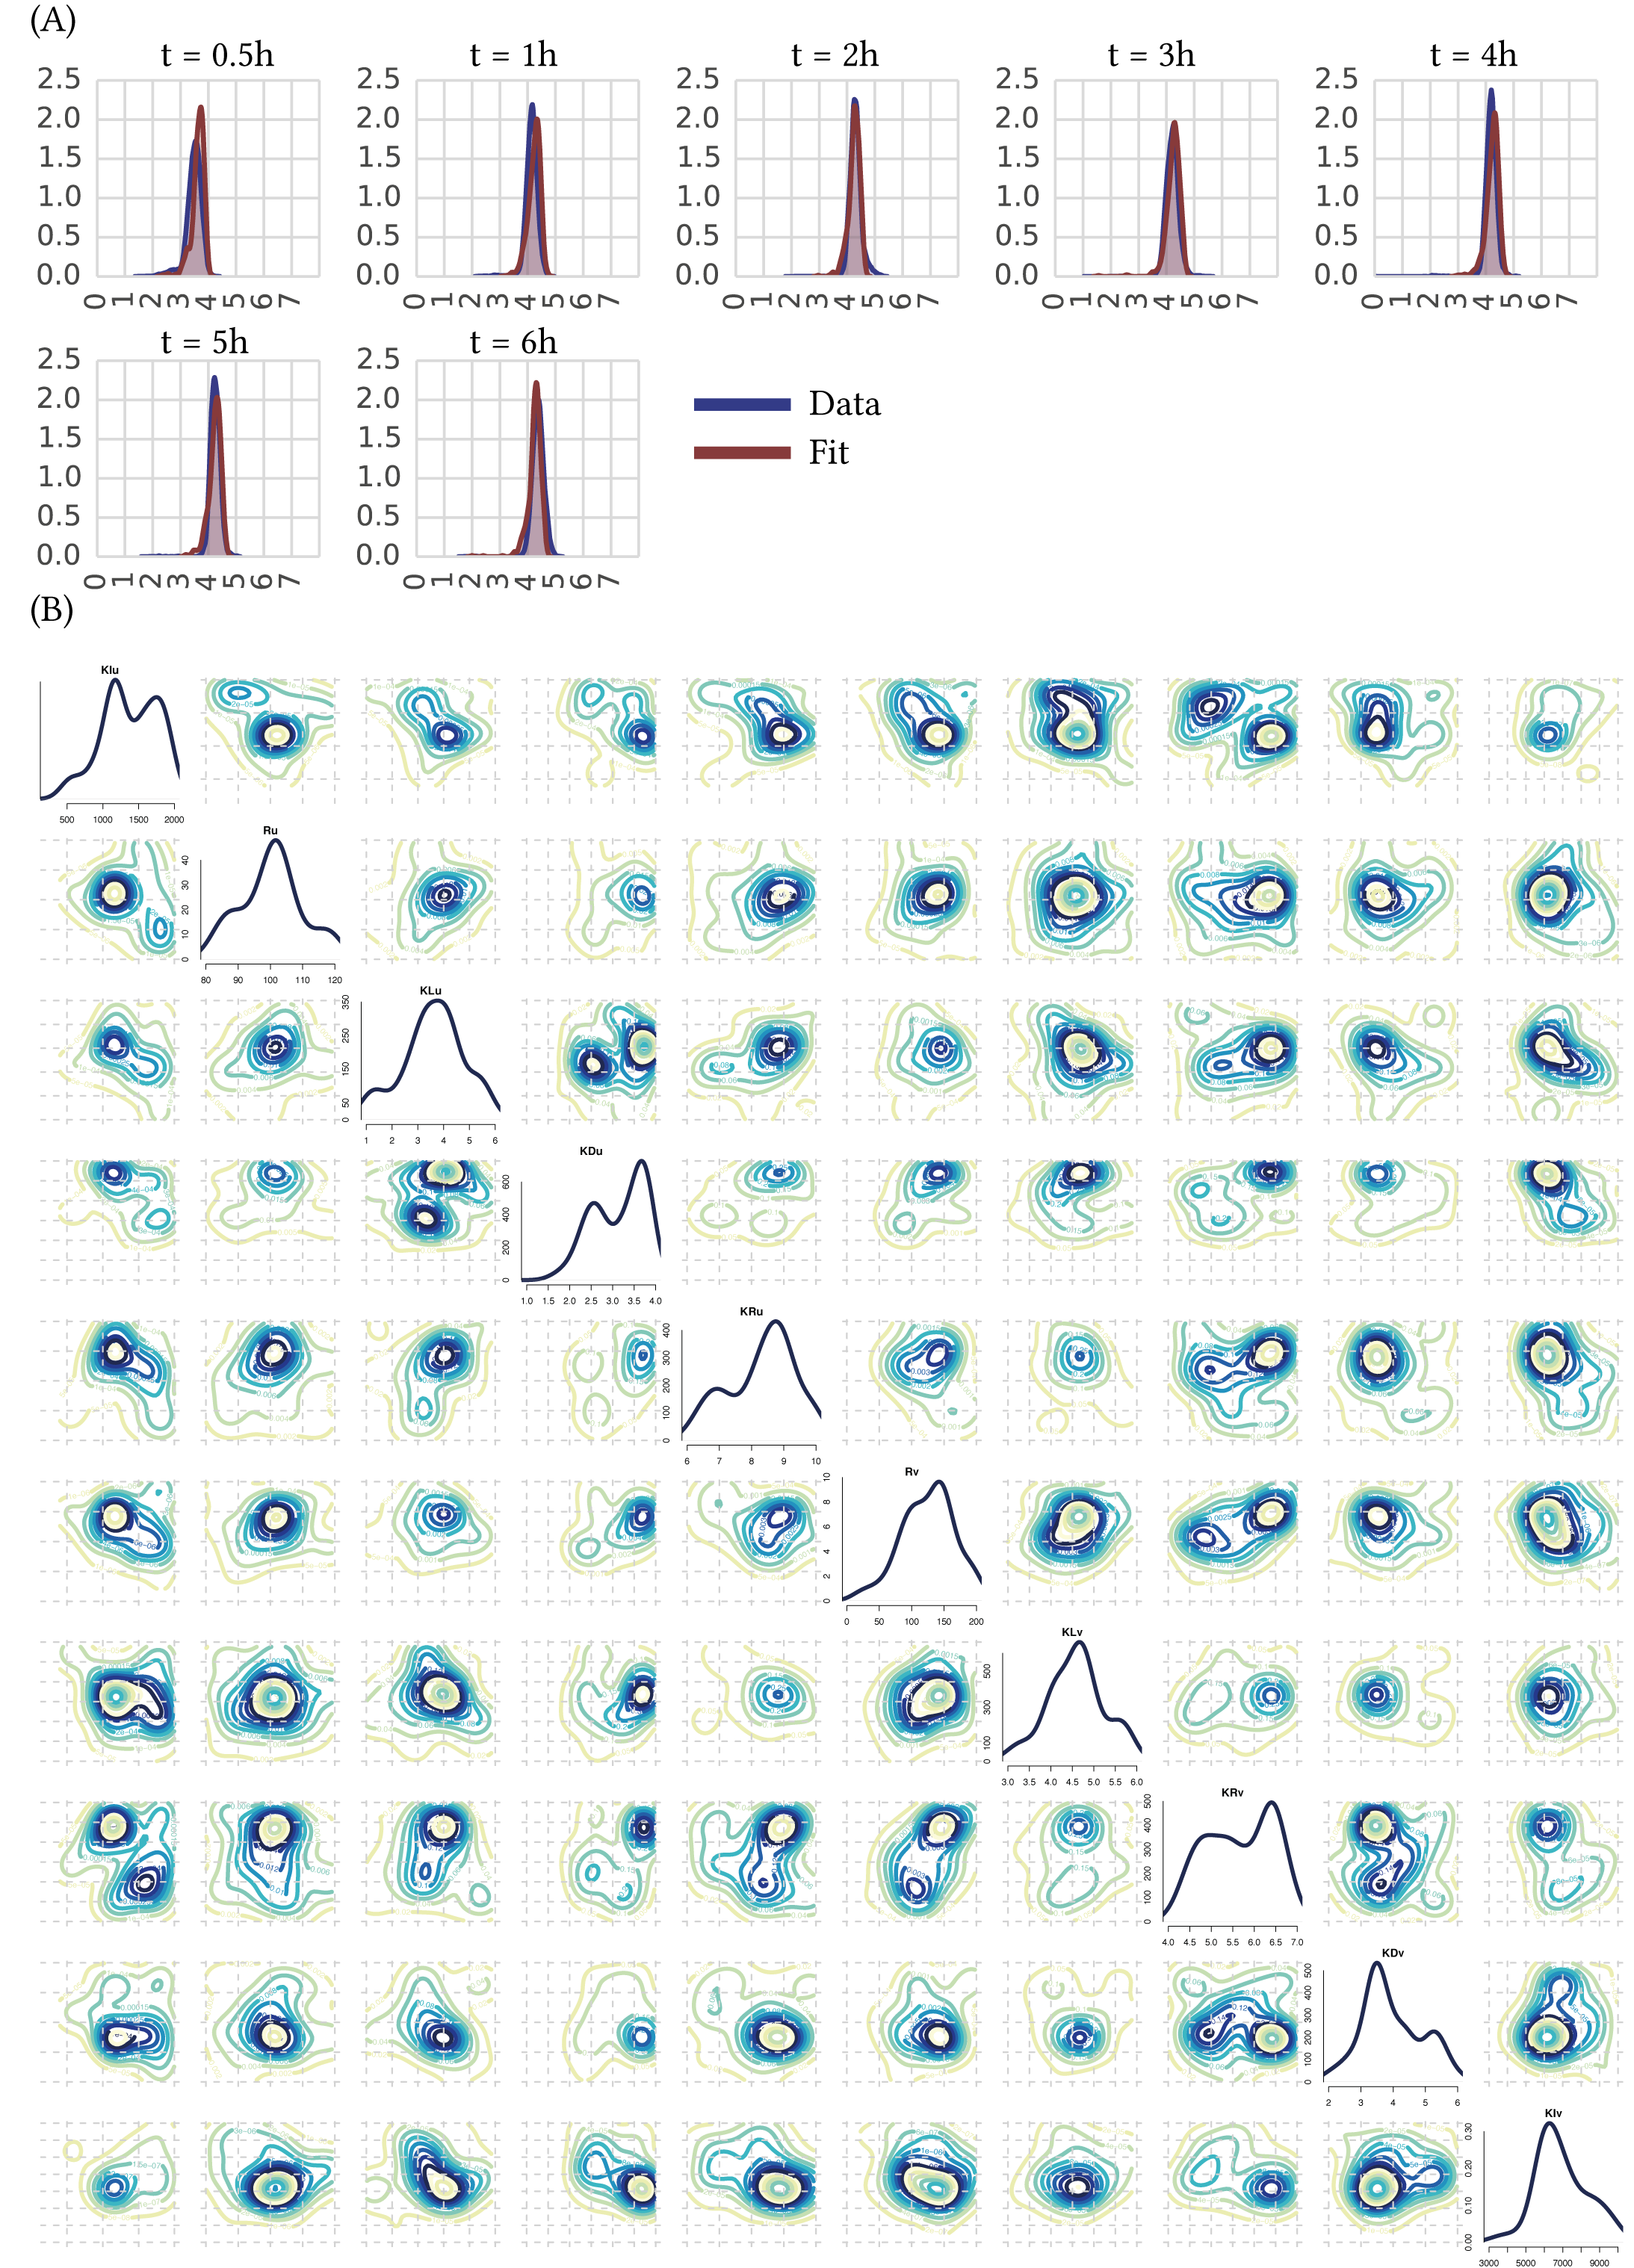
\includegraphics[scale=0.6]{chapterABCFlow/images/1D_real_res.png}
	\caption[LoF caption]{\label{fig:1d-real-res}}
\end{figure}




%\subsubsection{\acrshort{atc} induction}
 
 
%\begin{figure}[htbp]
%\centering
%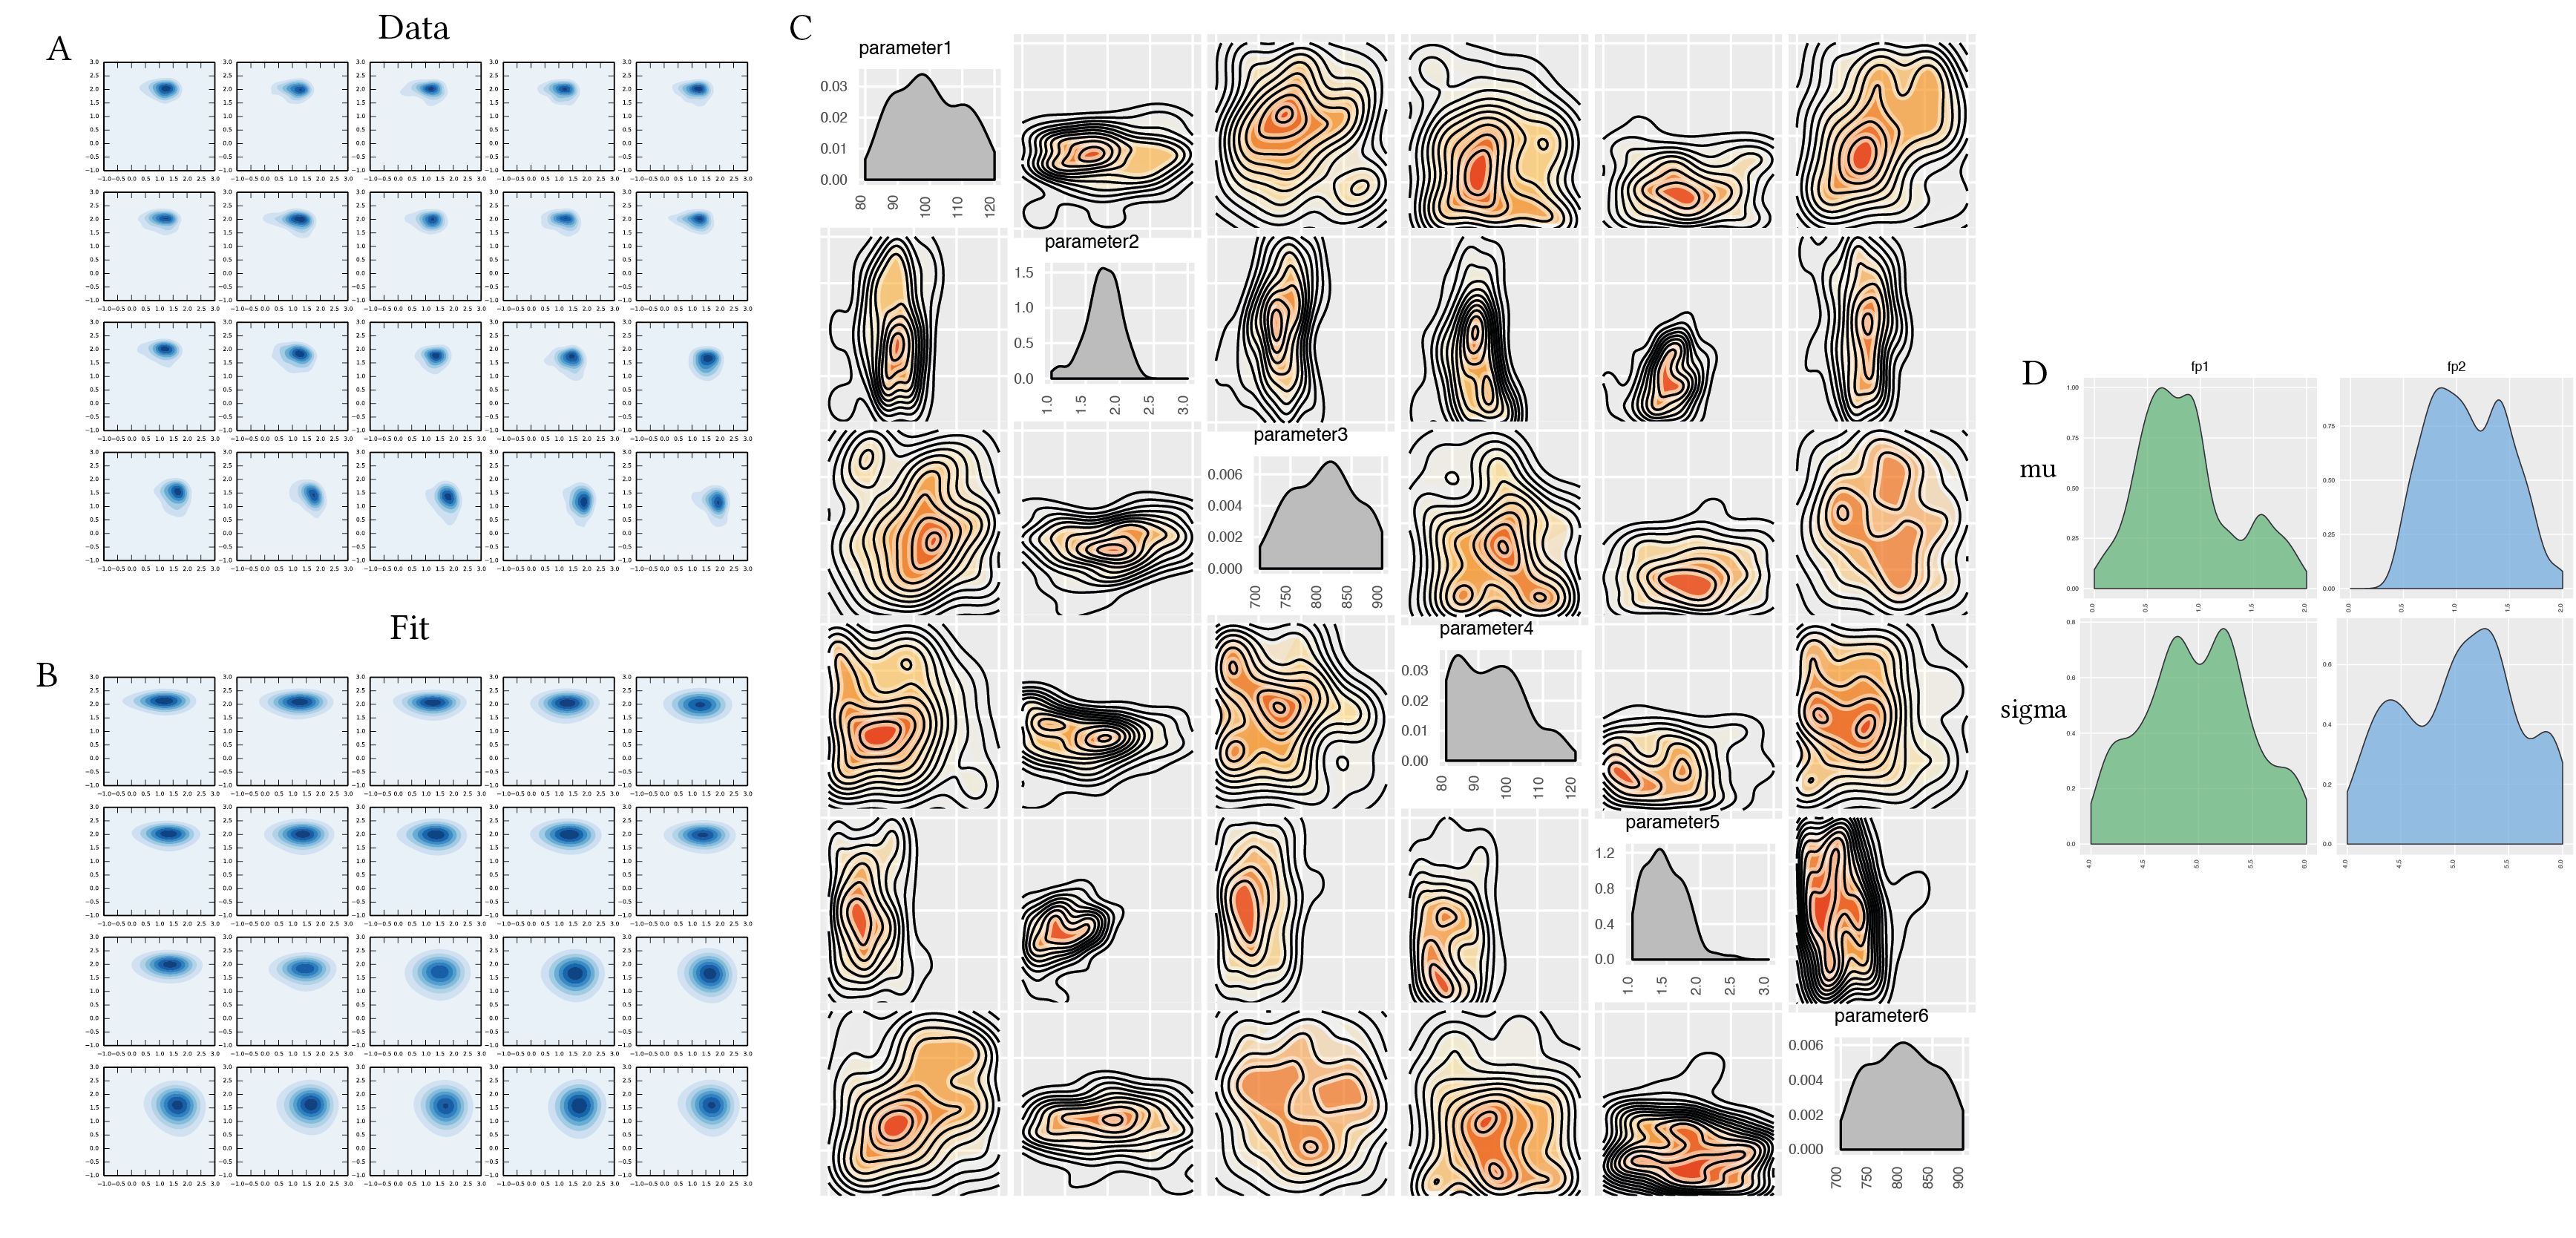
\includegraphics[scale=0.5]{chapterABCFlow/images/real_dat/real_dat_2D.png}
%\caption[LoF caption]{Real data 2D fit}
%\label{fig:real_dat_2d}
%\end{figure}
%\clearpage

%\subsubsection{\acrshort{iptg} induction}
\section{Discussion}

Here I characterised the genetic toggle switch experimentally. First I study the effect of the two inducers \acrshort{atc} and \acrshort{iptg} on the growth rate of the selected chassis \textit{E. coli} K-12 MG1655. I find that there is no detrimental effect to the bacterium by the inducers. I also find that which state the switch is on has no effect on the growth rate of the bacteria. In order for this toggle switch to be used in a synthetic biology application, it is important that both sides of the switch have an equivalent burden onto the chassis. If one of the steady states creates a larger burden and slows down the growth of the bacteria, this can create an imbalance in the population. If the toggle switch-bearing bacterial population exists in an environment with competing bacteria, for example the gut microbiome, and one of the two states creates a larger burden, this would cause the switch-bearing population to become less competitive compared to the non switch-bearing population. It is therefore crucial that the state of the switch does not affect the competitiveness of the chassis.  


I further characterised the switch by determining the minimum inducer concentration necessary to change the state of the switch. I find that for \acrshort{atc} induction, a minimum of \SI{0.09}{\nano\gram\per\milli\liter} is required to cause the switch to go to a GFP high state. For \acrshort{iptg} induction I find that a minimum of \SI{0.001}{M} is required to flip the switch to an mCherry high state. This information is critical for using this switch in other applications. Both sides of the switch are very sensitive to inducer concentrations, as the concentrations required to observe a change in fluorescence are very small. 

Furthermore I find that this toggle switch, pKDL071, is faster to respond to a change in \acrshort{atc} concentration that to a change in \acrshort{iptg} concentration. For \acrshort{iptg} induction we observe a change in fluorescence after 3-4 hours of induction. For \acrshort{atc} induction we can see a difference within an hour of induction. This result is in agreement with~\textcite{Litcofsky:2012gr}. This difference in response times must be taken into account when using the pKDL071 switch for other applications. This difference could be due to maturation times of the fluorescent proteins. \textcite{Macdonald:2012el} found that mCherry half-maturation time is 150 mins, whereas the GFP variant used here, GFPmut3b has been especially mutated for fast action~\autocite{Cormack:1996gv}. ~\textcite{Cormack:1996gv} found that whereas wild type GFP is detectable 1-2 hours after induction, GFPmut3b is detectable 8 minutes after induction. This difference could account for the different response times observed here, but further investigation is required. 


\section{Summary}


In this chapter I summarised the experiments carried out for the analysis of the genetic toggle switch. I used the pKDL071 plasmid and characterised its switching behaviour over various inducer concentrations and over time. I found the concentration of each inducer necessary to flip the switch as well as the time it takes for the change to be observed. Furthermore, I investigated the effect of the inducers on the growth rate of the chassis and found that they have no effect. In the next chapter I use the data collected in the chapter to fit to the more realistic toggle switch models used in Chapter (XXX). 





 
 